\documentclass{beamer}

\usetheme{CambridgeUS}
\usecolortheme{default}

% Definição de Cores - Carmesim Escuro / Vinho Profundo
\definecolor{main}{RGB}{139, 10, 35}         % Carmesim Escuro Profundo
\definecolor{darkmain}{RGB}{75, 5, 18}       % Carmesim Quase Negro / Vinho
\definecolor{background}{RGB}{255, 255, 255}

% Customização de Cores do Beamer
\setbeamercolor{palette primary}{bg=main, fg=white}
\setbeamercolor{palette secondary}{bg=darkmain, fg=white}
\setbeamercolor{palette tertiary}{bg=main, fg=white}
\setbeamercolor{titlelike}{fg=darkmain}
\setbeamercolor{block title}{bg=main, fg=white}
\setbeamercolor{block body}{bg=main!10, fg=black}
\setbeamercolor{item}{fg=main}

\usepackage[utf8]{inputenc}
\usepackage[T1]{fontenc}
\usepackage[brazil]{babel}
    % Customização de Cores do Beamer
    \setbeamercolor{palette primary}{bg=main, fg=white}
    \setbeamercolor{palette secondary}{bg=darkmain, fg=white}
    \setbeamercolor{palette tertiary}{bg=main, fg=white}
    \setbeamercolor{titlelike}{fg=darkmain}
    \setbeamercolor{block title}{bg=main, fg=white}
    \setbeamercolor{block body}{bg=main!10, fg=black}
    \setbeamercolor{item}{fg=main}

    \usepackage{csquotes}
    \usepackage{amsmath, amssymb, bm}
    \usepackage{booktabs}
    \usepackage{graphicx}
    \usepackage{algorithm2e}
    \usepackage{tikz}

    \usepackage[style=abnt, backend=biber, maxcitenames=2, mincitenames=1, maxbibnames=99, uniquelist=false, uniquename=false]{biblatex}
    \addbibresource{referencias.bib}

    \newcommand{\citep}[1]{\parencite{#1}}
    \newcommand{\citet}[1]{\textcite{#1}}

    \setbeamerfont{title}{size=\Large}

    % DADOS
    \title[NN-GLS \& INLA]{Estudo sobre Neural networks for geospatial data (NN-GLS)}
    \subtitle{Estimação de Parâmetros e Modelagem Espacial com INLA}
    \author[Pedro D. J. e Yuri D.]{Pedro Dresseno John e Yuri Dessimon}
    \institute[UFRGS]{
        Co-autroa: Profa. Dra. Márcia H. Barbian \\
        Departamento de Estatística \\
        Instituto de Matemática e Estatística \\
        Universidade Federal do Rio Grande do Sul (UFRGS)
    }
    \date{\today}

    \begin{document}

    % -------------------------------------------------------------
    % SLIDE 1: TÍTULO
    % -------------------------------------------------------------
    \begin{frame}[plain]
        \titlepage

        \begin{tikzpicture}[remember picture,overlay]
            % Logo FAPERGS (inferior esquerdo)
            % \node[
            %     anchor=south west,
            %     xshift=0cm,
            %     yshift=0cm               
            % ] at (current page.south west)
            % {
\includegraphics[height=2cm]{figuras/fapergs.jpg}};

            % Logo UFRGS (inferior direito)
            \node[
                anchor=south east,
                xshift=-1cm,
                yshift=0cm
            ] at (current page.south east)
            {
\includegraphics[height=2cm]{figuras/logo_ufrgs.png}};
        \end{tikzpicture}
    \end{frame}

    \begin{frame}{Séries Temporais como Processo Estocástico}

    \begin{block}{Definição}
    Uma série temporal é uma realização de um processo estocástico, isto é,
    uma coleção de variáveis aleatórias indexadas no tempo:

    \[
    \{X_t,\; t \in T\},
    \]

    em que cada \(X_t\) representa o valor observado da variável no instante \(t\).
    \end{block}

    \vspace{0.2cm}

    \begin{columns}[T]
    \column{0.55\textwidth}
    \textbf{Processo estocástico}

    \begin{itemize}
        \item O conjunto \(\{X_t\}\) é aleatório;
        \item Uma série observada é apenas uma realização;
        \item O objetivo é modelar a dependência entre os instantes de tempo.
    \end{itemize}

    \column{0.45\textwidth}
    \centering
    \begin{tikzpicture}[scale=0.8]
        % Eixos
        \draw[->] (0,0) -- (5.5,0) node[right] {\(t\)};
        \draw[->] (0,0) -- (0,3.2) node[above] {\(X_t\)};

        % Trajetória
        \draw[thick,blue]
            (0.3,1.2) --
            (0.8,1.8) --
            (1.3,1.4) --
            (1.8,2.3) --
            (2.3,1.7) --
            (2.8,2.6) --
            (3.3,2.1) --
            (3.8,2.8) --
            (4.3,2.4) --
            (4.8,2.9);

        % Pontos
        \foreach \x/\y in {0.3/1.2,0.8/1.8,1.3/1.4,1.8/2.3,2.3/1.7,2.8/2.6,3.3/2.1,3.8/2.8,4.3/2.4,4.8/2.9}
            \fill[blue] (\x,\y) circle (1.5pt);
    \end{tikzpicture}

    {\scriptsize Uma realização do processo}
    \end{columns}

    \vspace{0.3cm}

    \begin{alertblock}{Ideia central}
    A análise de séries temporais busca caracterizar a estrutura probabilística de
    \(X_t\), permitindo descrever, prever e inferir o comportamento futuro da série.
    \end{alertblock}

    \end{frame}

    \begin{frame}{Do Processo Temporal à um Processo Espacial}

    \begin{block}{Mesma ideia, índice diferente}
    Respostas $y(\bm{s})$ observadas como vesão ruidosa de um processo gaussiano $Z(\cdot) = \{Z(s) : s \subset R^2\}$.
    \end{block}

    \begin{columns}[T]
    %------------------- Temporal -------------------
    \column{0.48\textwidth}
    \centering
    \textbf{Série temporal}

    \vspace{0.2cm}

    \[
    \{X(t): t \in \mathbb{R}\}
    \]

    \begin{tikzpicture}[scale=0.75]
       % Eixos
        \draw[->] (0,0) -- (5.5,0) node[right] {\(t\)};
        \draw[->] (0,0) -- (0,3.2) node[above] {\(X_t\)};

        % Trajetória
        \draw[thick,blue]
            (0.3,1.2) --
            (0.8,1.8) --
            (1.3,1.4) --
            (1.8,2.3) --
            (2.3,1.7) --
            (2.8,2.6) --
            (3.3,2.1) --
            (3.8,2.8) --
            (4.3,2.4) --
            (4.8,2.9);

        % Pontos
        \foreach \x/\y in {0.3/1.2,0.8/1.8,1.3/1.4,1.8/2.3,2.3/1.7,2.8/2.6,3.3/2.1,3.8/2.8,4.3/2.4,4.8/2.9}
            \fill[blue] (\x,\y) circle (1.5pt);
    \end{tikzpicture}

    \[
    X(t) \sim GP\!\left(\mu(t),\, C(t,t')\right)
    \]

    {\scriptsize Dependência ao longo do tempo.}

    %------------------- Espacial -------------------
    \column{0.48\textwidth}
    \centering
    \textbf{Processo espacial}

    \vspace{0.2cm}

    \[
    \{Y(\mathbf{s}): \mathbf{s}\in\mathbb{R}^2\}
    \]

    \begin{tikzpicture}[scale=0.75]
        % eixos
        \draw[->] (0,0) -- (5.5,0) node[right] {\(x\)};
        \draw[->] (0,0) -- (0,3.2) node[above] {\(y\)};

        % pontos espaciais
        \foreach \x/\y in {
        0.5/0.5, 1.5/0.8, 2.7/0.4, 4.2/0.7,
        0.9/1.6, 2.1/1.3, 3.4/1.8, 4.7/1.4,
        1.3/2.6, 2.8/2.3, 4.0/2.7}
        \fill[red] (\x,\y) circle (2pt);
    \end{tikzpicture}

    \[
    Y(\mathbf{s}) \sim GP\!\left(\mu(\mathbf{s}),\, C(\mathbf{s},\mathbf{s}')\right)
    \]

    {\scriptsize Dependência entre localizações.}

    \end{columns}

    \end{frame}

\begin{frame}{Pressupostos do Processo Gaussiano}

    \begin{block}{Hipótese fundamental}
    Assume-se que a variável espacial é uma realização de um processo gaussiano
    $Z(s)$, de modo que qualquer conjunto finito de observações possui
    distribuição Normal multivariada.
    \end{block}

    \begin{columns}[T]

        \column{0.65\textwidth}

        \textbf{Pressupostos}

        \begin{itemize}
            \item Média: \(E[\mathbf{Y}] = \mathbf{X}\boldsymbol{\beta}\);
            \item Matriz de covariância: \(\boldsymbol{\Sigma}\);
            \item Dependência espacial modelada por \(C(\mathbf{h})\);
            \item Covariância depende do vetor de separação \(\mathbf{h}\) (Segunda Ordem) e/ou da distância \(\|\mathbf{h}\|\) (Instrinseca);
            \item O item anterior depende do tipo de estacionariedade assumida.
        \end{itemize}

        \column{0.35\textwidth}
        \centering

        \resizebox{\linewidth}{!}{$
        \mathbf{Y}=
        \begin{bmatrix}
        Y(\mathbf{s}_1)\\
        Y(\mathbf{s}_2)\\
        \vdots\\
        Y(\mathbf{s}_n)
        \end{bmatrix}
        \sim
        \mathcal{N}
        \left(
        \mathbf{X}\boldsymbol{\beta},
        \boldsymbol{\Sigma}
        \right)
        $}

    \end{columns}
\end{frame}

    \begin{frame}{Modelo Geoestatístico}
        \end{equation*}
        Usando o modelo geoestatístico:
        \begin{equation*}
            y(\bm{s}) = \mu(\bm{s}) + w(\bm{s}) + \epsilon(\bm{s})
        \end{equation*}
        onde:
        \begin{itemize}
            \item $\mu(\bm{s}) = \mathbf{X}\boldsymbol{\beta}$ é a tendência do processo em grande escala.
            \item $w(\bm{s}) \sim \mathcal{GP}(0, C(\cdot; \bm{\theta}))$ é um Processo Gaussiano de média zero que captura a dependência espacial de pequena escala.
            \item $\epsilon(\bm{s}) \stackrel{i.i.d.}{\sim} \mathcal{N}(0, \tau^2)$ efeito pepita.
        \end{itemize}

        \vspace{0.2cm}
        \begin{block}{Função de Covariância de Matérn}
            $C(h; \sigma^2, \kappa, \nu) = \frac{\sigma^2}{2^{\nu-1}\Gamma(\nu)} (\kappa h)^\nu K_\nu(\kappa h)$, onde $h = \|\bm{s}_i - \bm{s}_j\|$.
        \end{block}
    \end{frame}


    \begin{frame}{Contextualização e Motivação}
        \begin{itemize}
            \item \textbf{Contexto atual:}
            \begin{itemize}
                \item \emph{Modelos Geoestatísticos:} Modelam adequadamente a autocorrelação, porém a fórmula da tendências precisa ser especificada com antecedência;
                \item \emph{Redes Neurais Artificiais:} Capturam não linearidades e interações complexas dos preditores, mas violam a suposição de independência ($i.i.d.$) dos erros.
            \end{itemize}
            \item \textbf{Trabalho atual e o que fizemos de novo:} 
            \begin{itemize}
                \item Aplicar uma rede específica para dados espaciais;
                \item Modificação no método de estimação de parâmetros.
            \end{itemize}
        \end{itemize}
    \end{frame}

%\begin{frame}{O Gargalo da Máxima Verossimilhança (MLE)}
    %     Para $n$ localizações, o vetor de respostas $\bm{y} \sim \mathcal{N}(\bm{\mu}, \bm{\Sigma}(\bm{\theta}))$, onde:
    %     \begin{equation*}
    %         \bm{\Sigma}(\bm{\theta}) = \bm{C}_w(\sigma^2, \kappa) + \tau^2 \bm{I}_n
    %     \end{equation*}
        
    %     A log-verossimilhança do modelo é dada por:
    %     \begin{equation*}
    %         \ell(\bm{\mu}, \bm{\theta}) = -\frac{n}{2}\log(2\pi) - \frac{1}{2}\log|\bm{\Sigma}(\bm{\theta})| - \frac{1}{2}(\bm{y} - \bm{\mu})^\top \bm{\Sigma}(\bm{\theta})^{-1} (\bm{y} - \bm{\mu})
    %     \end{equation*}

    %     \begin{alertblock}{Complexidade Computacional ("Big $n$ Problem")}
    %         \begin{itemize}
    %             \item Inversão e determinante de $\bm{\Sigma}(\bm{\theta})$ exigem Decomposição de Cholesky com custo $\mathcal{O}(n^3)$ e memória $\mathcal{O}(n^2)$.
    %             \item Inviável para amostras moderadas a grandes ($n > 10^4$).
    %         \end{itemize}
    %     \end{alertblock}
    % \end{frame}

    % =============================================================
    % SEÇÃO 3: ABORDAGEM SPDE E INLA
    % =============================================================
    % \section{Abordagem SPDE \& INLA}

    % \begin{frame}{A Abordagem SPDE (Lindgren et al., 2011)}
    %     \begin{itemize}
    %         \item Um Campo Aleatório Gaussiano (GRF) contínuo com covariância de Matérn é a solução da Equação Diferencial Parcial Estocástica (SPDE):
    %         \begin{equation*}
    %             (\kappa^2 - \Delta)^{\alpha/2} (\tau w(\bm{s})) = \mathcal{W}(\bm{s})
    %         \end{equation*}
    %         \item \textbf{Discretização por Elementos Finitos (FEM):} O campo contínuo é representado sobre uma malha triangular (triangulação de Delaunay):
    %         \begin{equation*}
    %             w(\bm{s}) \approx \sum_{k=1}^{m} \psi_k(\bm{s}) \tilde{w}_k, \quad \tilde{\bm{w}} \sim \mathcal{N}(\bm{0}, \bm{Q}^{-1}(\bm{\theta}))
    %         \end{equation*}
    %     \end{itemize}
        
    %     \begin{block}{Propriedade Fundamental: Esparsidade}
    %         $\bm{Q}$ é uma \textbf{Matriz de Precisão Esparsa} (GMRF). O custo de fatoração cai de $\mathcal{O}(n^3)$ para $\mathcal{O}(n^{3/2})$ em 2D.
    %     \end{block}
    % \end{frame}

    % \begin{frame}{INLA (Integrated Nested Laplace Approximations)}
    %     \begin{columns}
    %         \begin{column}{0.5\textwidth}
    %             \begin{itemize}
    %                 \item Alternativa determinística rápida ao MCMC para Modelos Gaussianos Latentes (LGMs).
    %                 \item Utiliza aproximações de Laplace aninhadas para aproximar as marginais a posteriori:
    %                 \begin{align*}
    %                     p(\theta_k | \bm{y}) &\approx \int \tilde{p}(\bm{\theta} | \bm{y}) d\bm{\theta}_{-k} \\
    %                     p(x_i | \bm{y}) &\approx \int \tilde{p}(x_i | \bm{\theta}, \bm{y}) \tilde{p}(\bm{\theta} | \bm{y}) d\bm{\theta}
    %                 \end{align*}
    %             \end{itemize}
    %         \end{column}
            
    %         \begin{column}{0.5\textwidth}
    %             \begin{exampleblock}{Vantagens no Contexto Espacial}
    %                 \begin{itemize}
    %                     \item Convergência quase instantânea comparada ao Gibbs Sampler.
    %                     \item Estimativa direta dos hiperparâmetros espaciais $\bm{\theta} = (\sigma_w^2, \rho, \tau^2)$.
    %                     \item Integração direta com a matriz esparsa $\bm{Q}$.
    %                 \end{itemize}
    %             \end{exampleblock}
    %         \end{column}
    %     \end{columns}
    % \end{frame}

    % =============================================================
    % SEÇÃO 4: O MODELO NN-GLS
    % =============================================================
    \section{O Modelo NN-GLS}

\begin{frame}{Proposta do NN-GLS}

\begin{equation*}
\begin{aligned}
y(\mathbf{s}) &= f\!\left(X(\mathbf{s})\right)
              + w(\mathbf{s})
              + \epsilon(\mathbf{s}), \\
w(\cdot) &\sim GP\!\left(0,\Sigma(\cdot,\cdot)\right), \\
\epsilon(\cdot) &\sim \mathcal{N}(0, \tau^2).
\end{aligned}
\end{equation*}

\begin{itemize}
    \item Estimar $f(X(\mathbf{s}))$ usando uma rede neural que leva em conta a dependência espacial;
    \item Utilizar o Mínimos Quadrados Generalizados (MQG/GLS).
\end{itemize}

\begin{block}{Mínimos Quadrados Generalizados}
\[
\mathcal{L}_n(f)=
\frac{1}{n}
(\mathbf{Y}-f(\mathbf{X}))^\top
\boldsymbol{\Sigma ^{-1}}
(\mathbf{Y}-f(\mathbf{X})).
\]
\end{block}

\begin{block}{Mínimos Quadrados Ordinários}
\[
\mathcal{L}_n(f) = 
\frac{1}{n}
(\mathbf{Y}-f(\mathbf{X}))^\top 
(\mathbf{Y}-f(\mathbf{X})).
\]
\end{block}
\end{frame}

\begin{frame}{Desafio da proposta}
    \begin{itemize}
        \item GLS não é compatível com a técnica de mini-batching por não possuir aditividade como OLS;
        \item Back-propagation envolve a inversão de uma matriz $n \times n$ que requer $\mathcal{O}(n^2)$ espaço de memória e $\mathcal{O}(n^3)$ tempo de cada interação;
    \end{itemize}

    \begin{block}{}
    \centering
    \Large\bfseries
    Como o artigo contornou esses problemas?
    \end{block}

%     \begin{block}{kek}
        
%     \end{block}

%     \begin{block}{A Solução: Perda OLS Decorrelacionada}
%         Fatorando a matriz de precisão via Cholesky ($\bm{\Sigma}^{-1} = \bm{L}^\top \bm{L}$), podemos demonstrar que a perda GLS é matematicamente equivalente à perda OLS (MSE) aplicada sobre os dados transformados:
%         \begin{equation*}
%             \mathcal{L}_{GLS} = (\bm{y} - \hat{\bm{y}})^\top (\bm{L}^\top \bm{L}) (\bm{y} - \hat{\bm{y}}) = \| \underbrace{\bm{L}\bm{y}}_{\tilde{\bm{y}}} - \underbrace{\bm{L}\hat{\bm{y}}}_{\tilde{\hat{\bm{y}}}} \|^2 = \mathcal{L}_{OLS}(\tilde{\bm{y}}, \tilde{\hat{\bm{y}}})
%         \end{equation*}
%     \end{block}
\end{frame}

\begin{frame}{Como o artigo contornou esse problema?}

    \begin{block}{Ideia central}
        \begin{itemize}
            \item Utilizar o \textbf{Nearest Neighbor Gaussian Process (NNGP)} que reduz a complexidade computacional ao calcularmos $\Sigma$ apenas com os vizinhos mais próximos;
            \item Transformar o problema de GLS em um problema equivalente de OLS.
        \end{itemize}
    \end{block}


    \begin{center}
        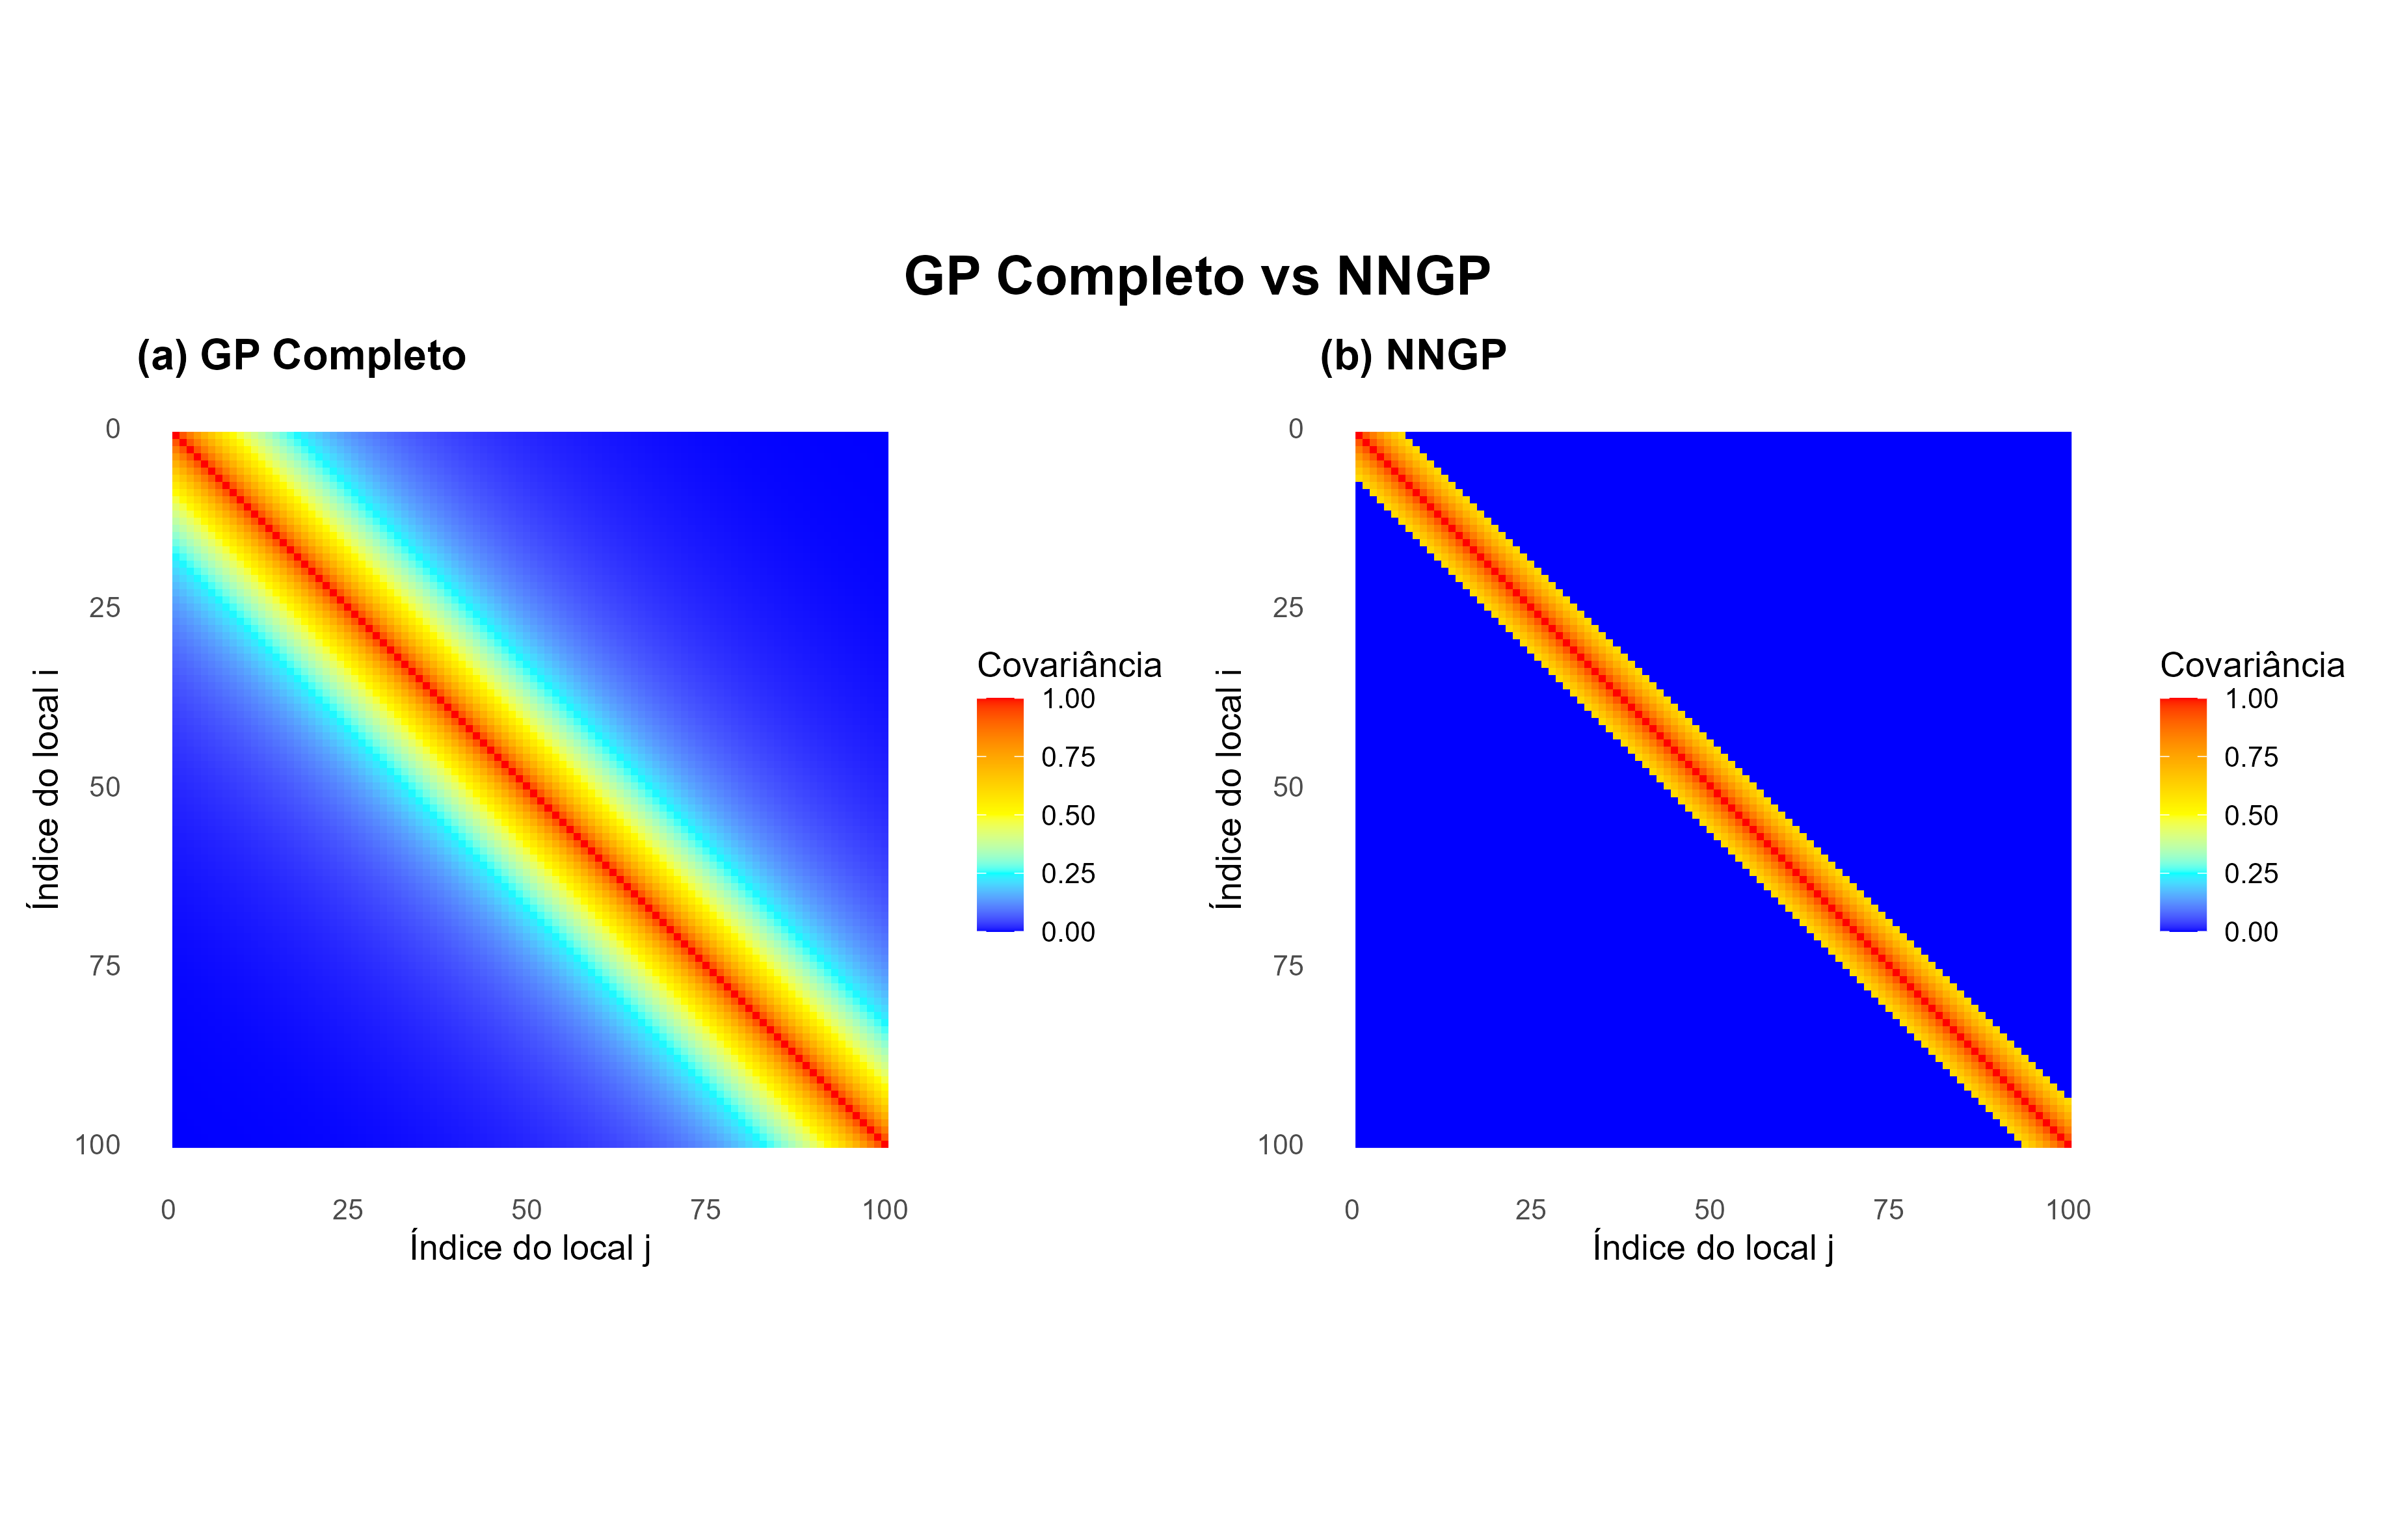
\includegraphics[width=0.7\textwidth]{figuras/nngpxgp.png}
    \end{center}

\end{frame}

\begin{frame}
    \begin{block}{Ideia central}
        Uma perda GLS pode ser vista como uma perda OLS para a resposta descorrelacionada $\boldsymbol{Y}^* = \mathbf{Q}^{\frac{1}{2}}\boldsymbol{Y}$, 
        em que $\mathbf{Q}^{\frac{1}{2}}$ é o fator de Cholesky de $\mathbf{Q} = \mathbf{Q}^{\frac{\top}{2}}\mathbf{Q}^{\frac{1}{2}}$.
    \end{block}
    \vspace{0.2cm}

    Para trabalharmos com GLS o artigo propõe a transformação acima que decorrelaciona as respostas. Logo a rede vira:
    \vspace{0.2cm}

    \begin{enumerate}
        \item Decorrelação espacial (com de parâmetros iniciais da func de covariância);
        \item Treinamento de MLP;
        \item Camada de output da MLP é uma convolução;
        \item Cálculo dos resíduos;
        \item Depois de fazer backpropagation um número M de vezes, estimar os parâmetros novamente. 
    \end{enumerate}
\end{frame}


%-------------------------------------------------
\begin{frame}{Estimação dos Parâmetros Espaciais}

\begin{block}{Objetivo}
Estimar os parâmetros da matriz de covariância
\[
\theta=(\sigma^2,\phi,\tau^2),
\]
utilizando os resíduos produzidos pela rede neural.
\end{block}

\[
\mathbf{w}=\mathbf{y}-\hat{\mathbf{y}}
\]

\begin{itemize}
    \item A MLP estima apenas a média não linear $f(\mathbf{x})$;
    \item A dependência espacial permanece nos resíduos $\mathbf{w}$;
    \item A cada época, os parâmetros espaciais são reestimados e uma nova matriz $\Sigma(\theta)$ é construída.
\end{itemize}

\begin{center}
MLP $\rightarrow$ Resíduos $\rightarrow$ Estimação de $\theta$ $\rightarrow$ Nova $\Sigma$
\end{center}

\end{frame}

%-------------------------------------------------
\begin{frame}{Estimação por BRISC}

\begin{block}{Ideia principal}
O BRISC estima $\theta=(\sigma^2,\phi,\tau^2)$ por Máxima Verossimilhança utilizando a aproximação do NNGP.
\end{block}

A log-verossimilhança aproximada é dada por

\[
\ell(\theta)=
-\frac{1}{2}
\sum_{i=1}^{n}
\left[
\log(F_i)+
\frac{(w_i-\mathbf{B}_i\mathbf{w}_{N_i})^2}{F_i}
\right].
\]

\begin{itemize}
    \item Constrói vizinhos mais próximos para cada observação;
    \item Evita inverter a matriz $\Sigma_{n\times n}$ completa;
    \item Complexidade aproximadamente linear em $n$;
    \item Retorna estimativas MLE de $\sigma^2$, $\phi$ e $\tau^2$.
\end{itemize}

\end{frame}

%-------------------------------------------------
\begin{frame}{Estimação Bayesiana por INLA}

\begin{block}{Ideia principal}
O INLA obtém a distribuição posterior dos parâmetros espaciais sem utilizar MCMC.
\end{block}

Modelo hierárquico:

\[
\mathbf{w}\mid\theta
\sim
\mathcal{N}(0,\Sigma(\theta))
\]

\[
\pi(\theta\mid\mathbf{w})
\propto
\pi(\mathbf{w}\mid\theta)\,
\pi(\theta)
\]

O INLA aproxima numericamente as distribuições posteriores de

\[
\sigma^2,\qquad
\phi,\qquad
\tau^2.
\]

\begin{itemize}
    \item Inferência Bayesiana rápida por aproximações de Laplace;
    \item Fornece média, moda, desvio padrão e intervalos de credibilidade;
    \item Permite quantificar a incerteza dos parâmetros espaciais.
\end{itemize}

\end{frame}

    % \begin{frame}{Integração NN-GLS com INLA/SPDE}
    %     \begin{block}{Otimização em Duas Etapas Iterativas}
    %         Como $\bm{\Sigma}(\bm{\theta})^{-1} \approx \bm{A}^\top \bm{Q}(\bm{\theta}) \bm{A} + \tau^{-2}\bm{I}$, alternamos entre:
    %     \end{block}

    %     \begin{enumerate}
    %         \item \textbf{Passo 1: Treinamento da Rede Neural ($f_{\bm{\Theta}}$)}
    %         \begin{itemize}
    %             \item Fixa-se $\bm{\theta}$ (e a matriz de precisão $\bm{Q}$).
    %             \item Atualiza-se os pesos da rede $\bm{\Theta}_{NN}$ via Gradiente Descendente utilizando a perda GLS espacialmente decorrelacionada.
    %         \end{itemize}
            
    %         \item \textbf{Passo 2: Estimação Espacial via INLA ($\bm{\theta}$)}
    %         \begin{itemize}
    %             \item Calcula-se o resíduo da rede: $\bm{r} = \bm{y} - f_{\bm{\Theta}_{NN}}(\bm{X})$.
    %             \item Ajusta-se o modelo espacial $\bm{r} = \bm{A}\tilde{\bm{w}} + \bm{\epsilon}$ via **R-INLA** para obter a estimativa a posteriori (ou moda marginal) dos parâmetros de Matérn $\hat{\bm{\theta}} = (\hat{\sigma}^2, \hat{\kappa}, \hat{\tau}^2)$.
    %         \end{itemize}
    %     \end{enumerate}
    % \end{frame}

    % \begin{frame}{Fluxo do Algoritmo NN-GLS + INLA}
    %     \begin{center}
    %         \fbox{\parbox{0.9\textwidth}{
    %             \textbf{Algoritmo: NN-GLS com INLA/SPDE}
    %             \begin{enumerate}
    %                 \item Construir malha FEM nos nós espaciais $\bm{s}_1, \dots, \bm{s}_n$ e matriz projetora $\bm{A}$.
    %                 \item Inicializar pesos da rede neural $\bm{\Theta}_{NN}^{(0)}$ e resíduos $\bm{r}^{(0)} = \bm{y}$.
    %                 \item \textbf{Para} $k = 1, \dots, K_{\max}$ \textbf{faça}:
    %                 \begin{itemize}
    %                     \item Executar INLA sobre $\bm{r}^{(k-1)}$ $\rightarrow$ Obter $\bm{Q}(\hat{\bm{\theta}}^{(k)})$ e $\hat{\bm{w}}^{(k)}$.
    %                     \item Definir operador de decorrelação $\bm{L}^{(k)}$ onde $\bm{L}^\top \bm{L} \approx \bm{\Sigma}(\hat{\bm{\theta}}^{(k)})^{-1}$.
    %                     \item Treinar rede em $\tilde{\bm{y}} = \bm{L}\bm{y}$ com entradas $\tilde{\bm{X}}$ $\rightarrow$ Obter $\bm{\Theta}_{NN}^{(k)}$.
    %                     \item Atualizar resíduos: $\bm{r}^{(k)} = \bm{y} - f_{\bm{\Theta}_{NN}^{(k)}}(\bm{X})$.
    %                     \item Verificar critério de convergência $\|\hat{\bm{\theta}}^{(k)} - \hat{\bm{\theta}}^{(k-1)}\| < \epsilon$.
    %                 \end{itemize}
    %                 \item \textbf{Retornar:} Preditor espacial combinado $\hat{y}(\bm{s}_0) = f_{\hat{\bm{\Theta}}}(\bm{x}(\bm{s}_0)) + \hat{w}(\bm{s}_0)$.
    %             \end{enumerate}
    %         }}
    %     \end{center}
    % \end{frame}

    % =============================================================
    % SEÇÃO 5: RESULTADOS E COMPARAÇÕES
    % =============================================================
    \section{Resultados}

\begin{frame}{Estudo de Simulação}
    \begin{itemize}
        \item Foi usada a função grf() do pacote geoR;
        \item Função de covariância Matérn ($\nu = 1$);
        \item \textbf{Geração dos Dados:}
        \item coordenadas $\sim$ runif(0,10)
        \item $\mathbf X \sim$ unif(0,1) 
        \begin{equation*}
            \mu(s) = \frac{1}{6}(10 \sin(\pi x_1(s) x_2(s)) + 20(x_3(s) - 0.5)^2 + 10 x_4(s) + 5 x_5(s))
        \end{equation*}
        \item \textbf{Cenários Amostrais - INLA:} $n = 2000$
        \begin{itemize}
            \item \textbf{Variância Espacial ($\sigma^2$):} $\{0.5,\, 1.0,\, 5.0,\, 10.0,\, 20.0\}$
            \item \textbf{Alcance Espacial $\cdot \sqrt{2}$:} $\{0.5,\, 1,\, 3,\, 6,\, 12\}$
            \item \textbf{Pepita: $\tau^2 = 0.1 \cdot \sigma^2$}
        \end{itemize}
    \end{itemize}
\end{frame}

\begin{frame}{Resultados Comparativos}
    \begin{center}
        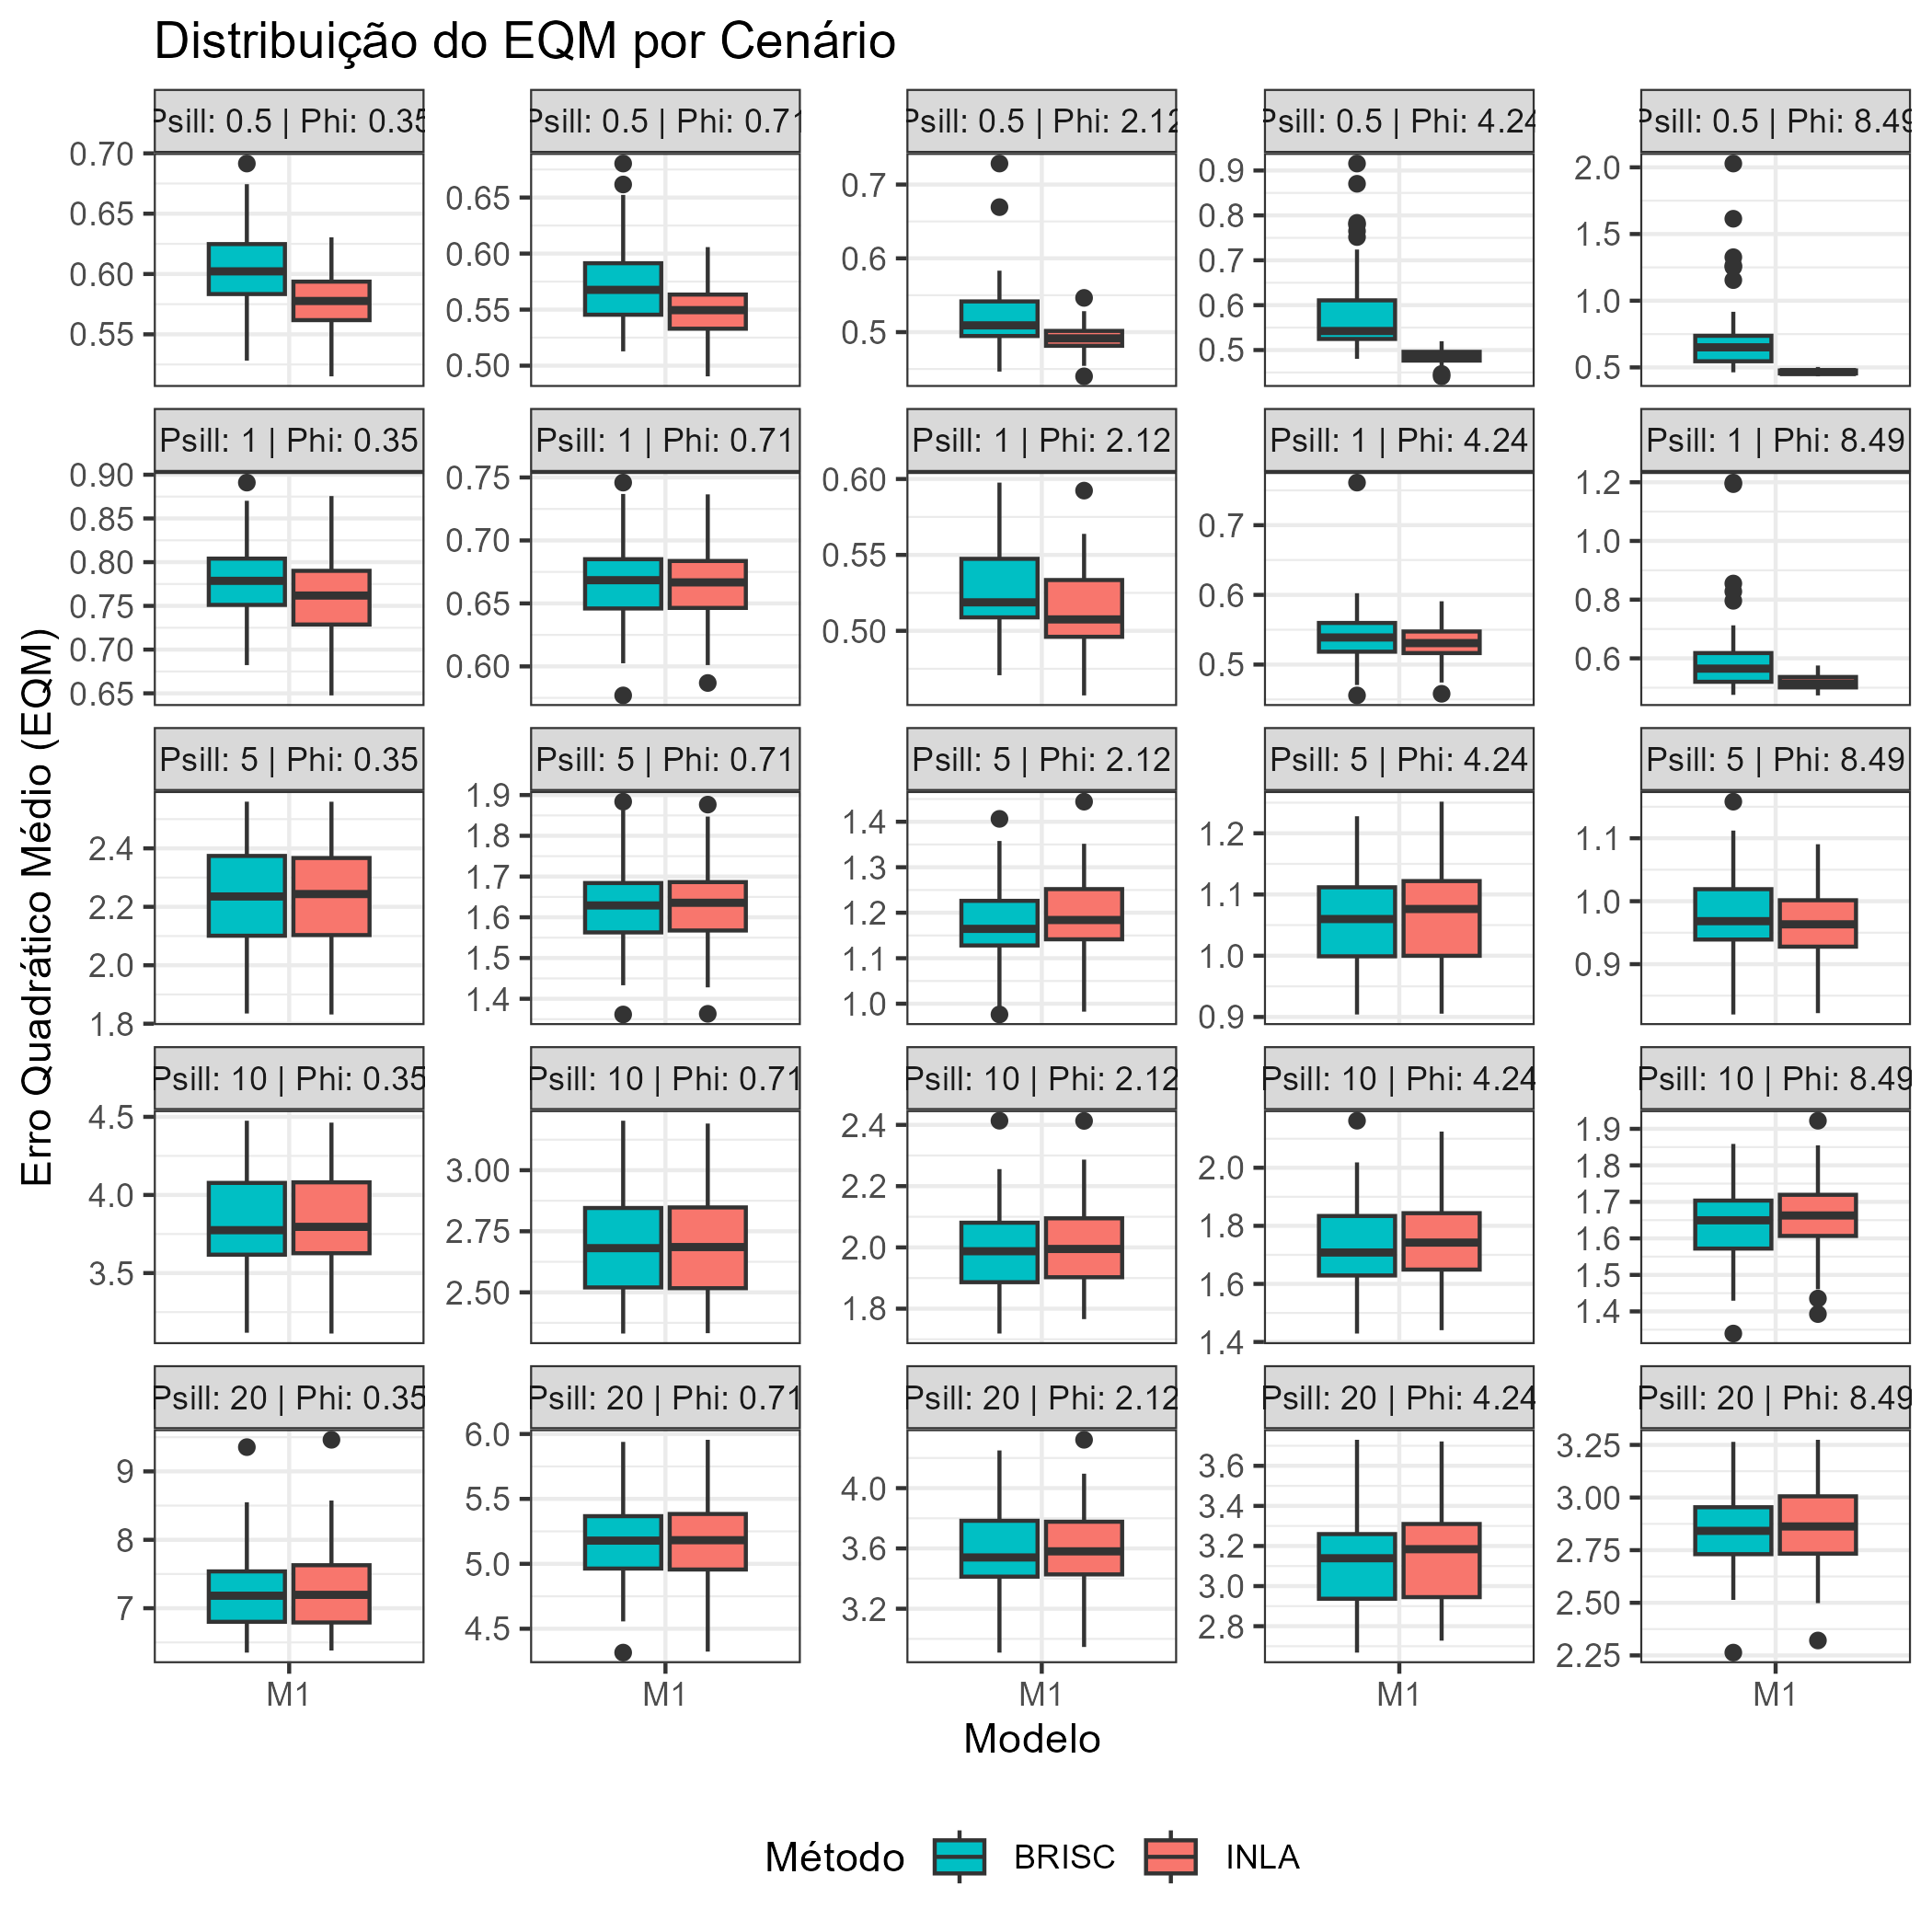
\includegraphics[width=0.7\textwidth]{figuras/eqm_cen.png}
    \end{center}
\end{frame}

\begin{frame}
\begin{table}[htbp]
    \centering
    \small
    \label{tabela_resultados_slides}
    \resizebox{\textwidth}{!}{%
    \begin{tabular}{@{}ccccccccc@{}}
        \toprule
        $\sigma^2_{\text{real}}$ & $\phi_{\text{real}}$ & EQM Bayes & EQM Freq & Média $\Delta$ & DP $\Delta$ & Mín $\Delta$ & Máx $\Delta$ & \% Bayes Melhor \\
        \midrule
        0.5 & $\frac{0.5}{\sqrt{2}}$  & 0.577 & 0.604 &  0.0274 & 0.0184 & -0.0036 & 0.0786 & 98 \\
        0.5 & $\frac{3}{\sqrt{2}}$    & 0.492 & 0.521 &  0.0294 & 0.0462 & -0.0102 & 0.2503 & 84 \\
        0.5 & $\frac{12}{\sqrt{2}}$   & 0.465 & 0.731 &  0.2655 & 0.3017 &  0.0068 & 1.5456 & 100 \\
        \addlinespace
        1.0 & $\frac{0.5}{\sqrt{2}}$  & 0.760 & 0.777 &  0.0169 & 0.0108 & -0.0021 & 0.0482 & 98 \\
        1.0 & $\frac{3}{\sqrt{2}}$    & 0.514 & 0.530 &  0.0160 & 0.0143 & -0.0096 & 0.0563 & 94 \\
        1.0 & $\frac{12}{\sqrt{2}}$   & 0.519 & 0.607 &  0.0876 & 0.1447 & -0.0068 & 0.6935 & 98 \\
        \addlinespace
        5.0 & $\frac{0.5}{\sqrt{2}}$  & 2.230 & 2.230 &  0.0011 & 0.0087 & -0.0196 & 0.0319 & 54 \\
        5.0 & $\frac{3}{\sqrt{2}}$    & 1.190 & 1.180 & -0.0129 & 0.0161 & -0.0620 & 0.0171 & 22 \\
        5.0 & $\frac{12}{\sqrt{2}}$   & 0.963 & 0.976 &  0.0126 & 0.0396 & -0.0257 & 0.2303 & 60 \\
        \addlinespace
        10.0 & $\frac{0.5}{\sqrt{2}}$ & 3.840 & 3.830 & -0.0094 & 0.0227 & -0.0670 & 0.0373 & 40 \\
        10.0 & $\frac{3}{\sqrt{2}}$   & 2.010 & 2.000 & -0.0169 & 0.0212 & -0.0805 & 0.0241 & 20 \\
        10.0 & $\frac{12}{\sqrt{2}}$  & 1.660 & 1.640 & -0.0196 & 0.0219 & -0.0635 & 0.0159 & 18 \\
        \addlinespace
        20.0 & $\frac{0.5}{\sqrt{2}}$ & 7.280 & 7.260 & -0.0213 & 0.0565 & -0.1245 & 0.1019 & 36 \\
        20.0 & $\frac{3}{\sqrt{2}}$   & 3.600 & 3.580 & -0.0294 & 0.0346 & -0.1337 & 0.0516 & 20 \\
        20.0 & $\frac{12}{\sqrt{2}}$  & 2.860 & 2.840 & -0.0215 & 0.0393 & -0.1277 & 0.0445 & 26 \\
        \bottomrule
    \end{tabular}%
    }
\end{table}
\end{frame}

% \begin{frame}{Resultados Comparativos}
%     \begin{itemize}
%         \item Clara relação entre a porcentagem de "vitórias" da estimação bayesiana com a dependência espacial;
%         \item Leve relação com o $phi$;
%         \item Vitórias do INLA são mais expressivas.
%     \end{itemize}
%     \begin{center}
%         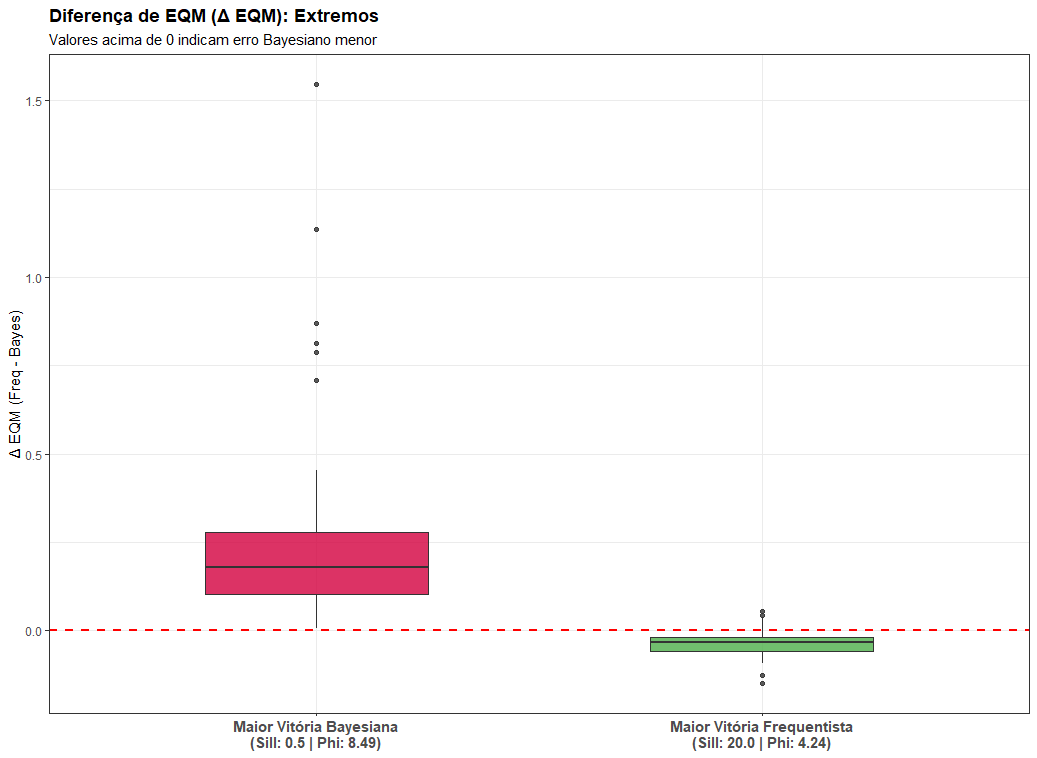
\includegraphics[width=0.5\textwidth]{figuras/EQM_Extremos.png}
%     \end{center}
% \end{frame}

\begin{frame}{Resultados Comparativos}

\begin{columns}[c]
    \column{0.52\textwidth}

    \begin{itemize}
        \item Clara relação entre a porcentagem de vitórias da estimação Bayesiana e a dependência espacial;
        \item Leve relação com o parâmetro $\phi$;
        \item As vitórias do INLA são mais expressivas.
    \end{itemize}

    \column{0.48\textwidth}
    \centering
    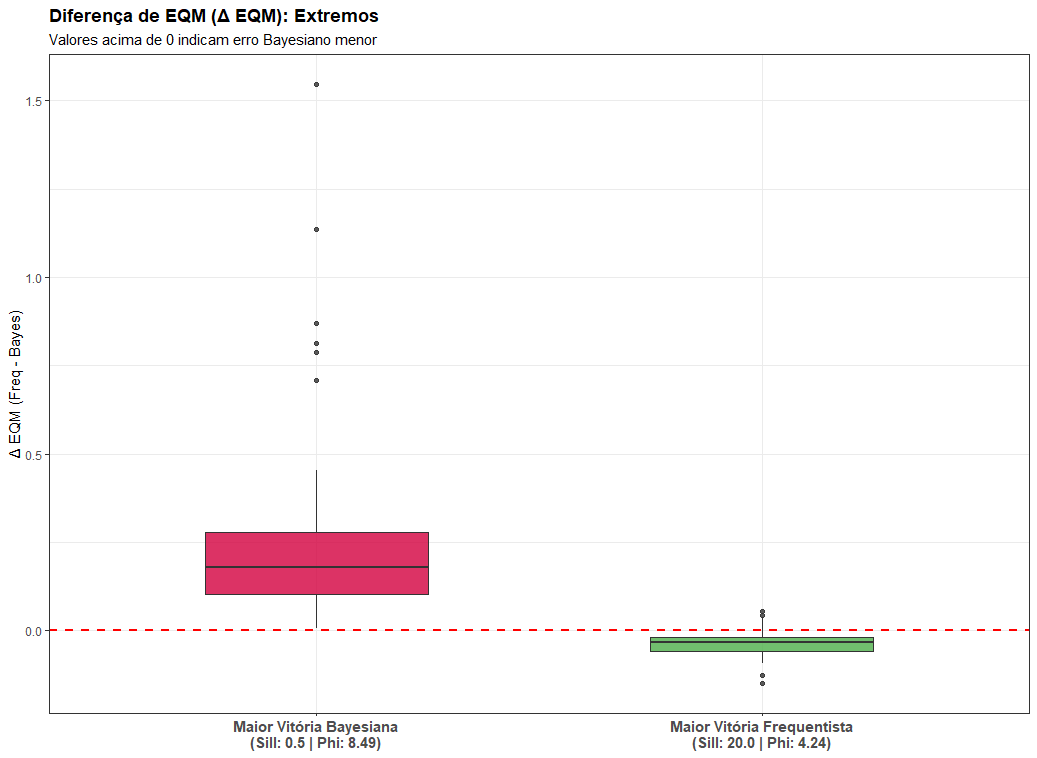
\includegraphics[width=\linewidth]{figuras/EQM_Extremos.png}
\end{columns}

\end{frame}

% \begin{frame}{Dados}
%     \begin{itemize}
%         \item Banco de dados na região do norte da Tanzânia e outros países próximos;
%         \item Decidimos trabalhar apenas com dados das regiões: Mwanza, Geita, Simiyu, Mara e Shinyanga;
%         \item Variável resposta: pH ;
%         \item Covariáveis: Carbono total, Nitrogênio, Alumínio, Cálcio, Cobre, Ferro, Manganês, Magnésio e Potássio (e Latitude e Longitude).
%     \end{itemize} 
%         \begin{center}
%         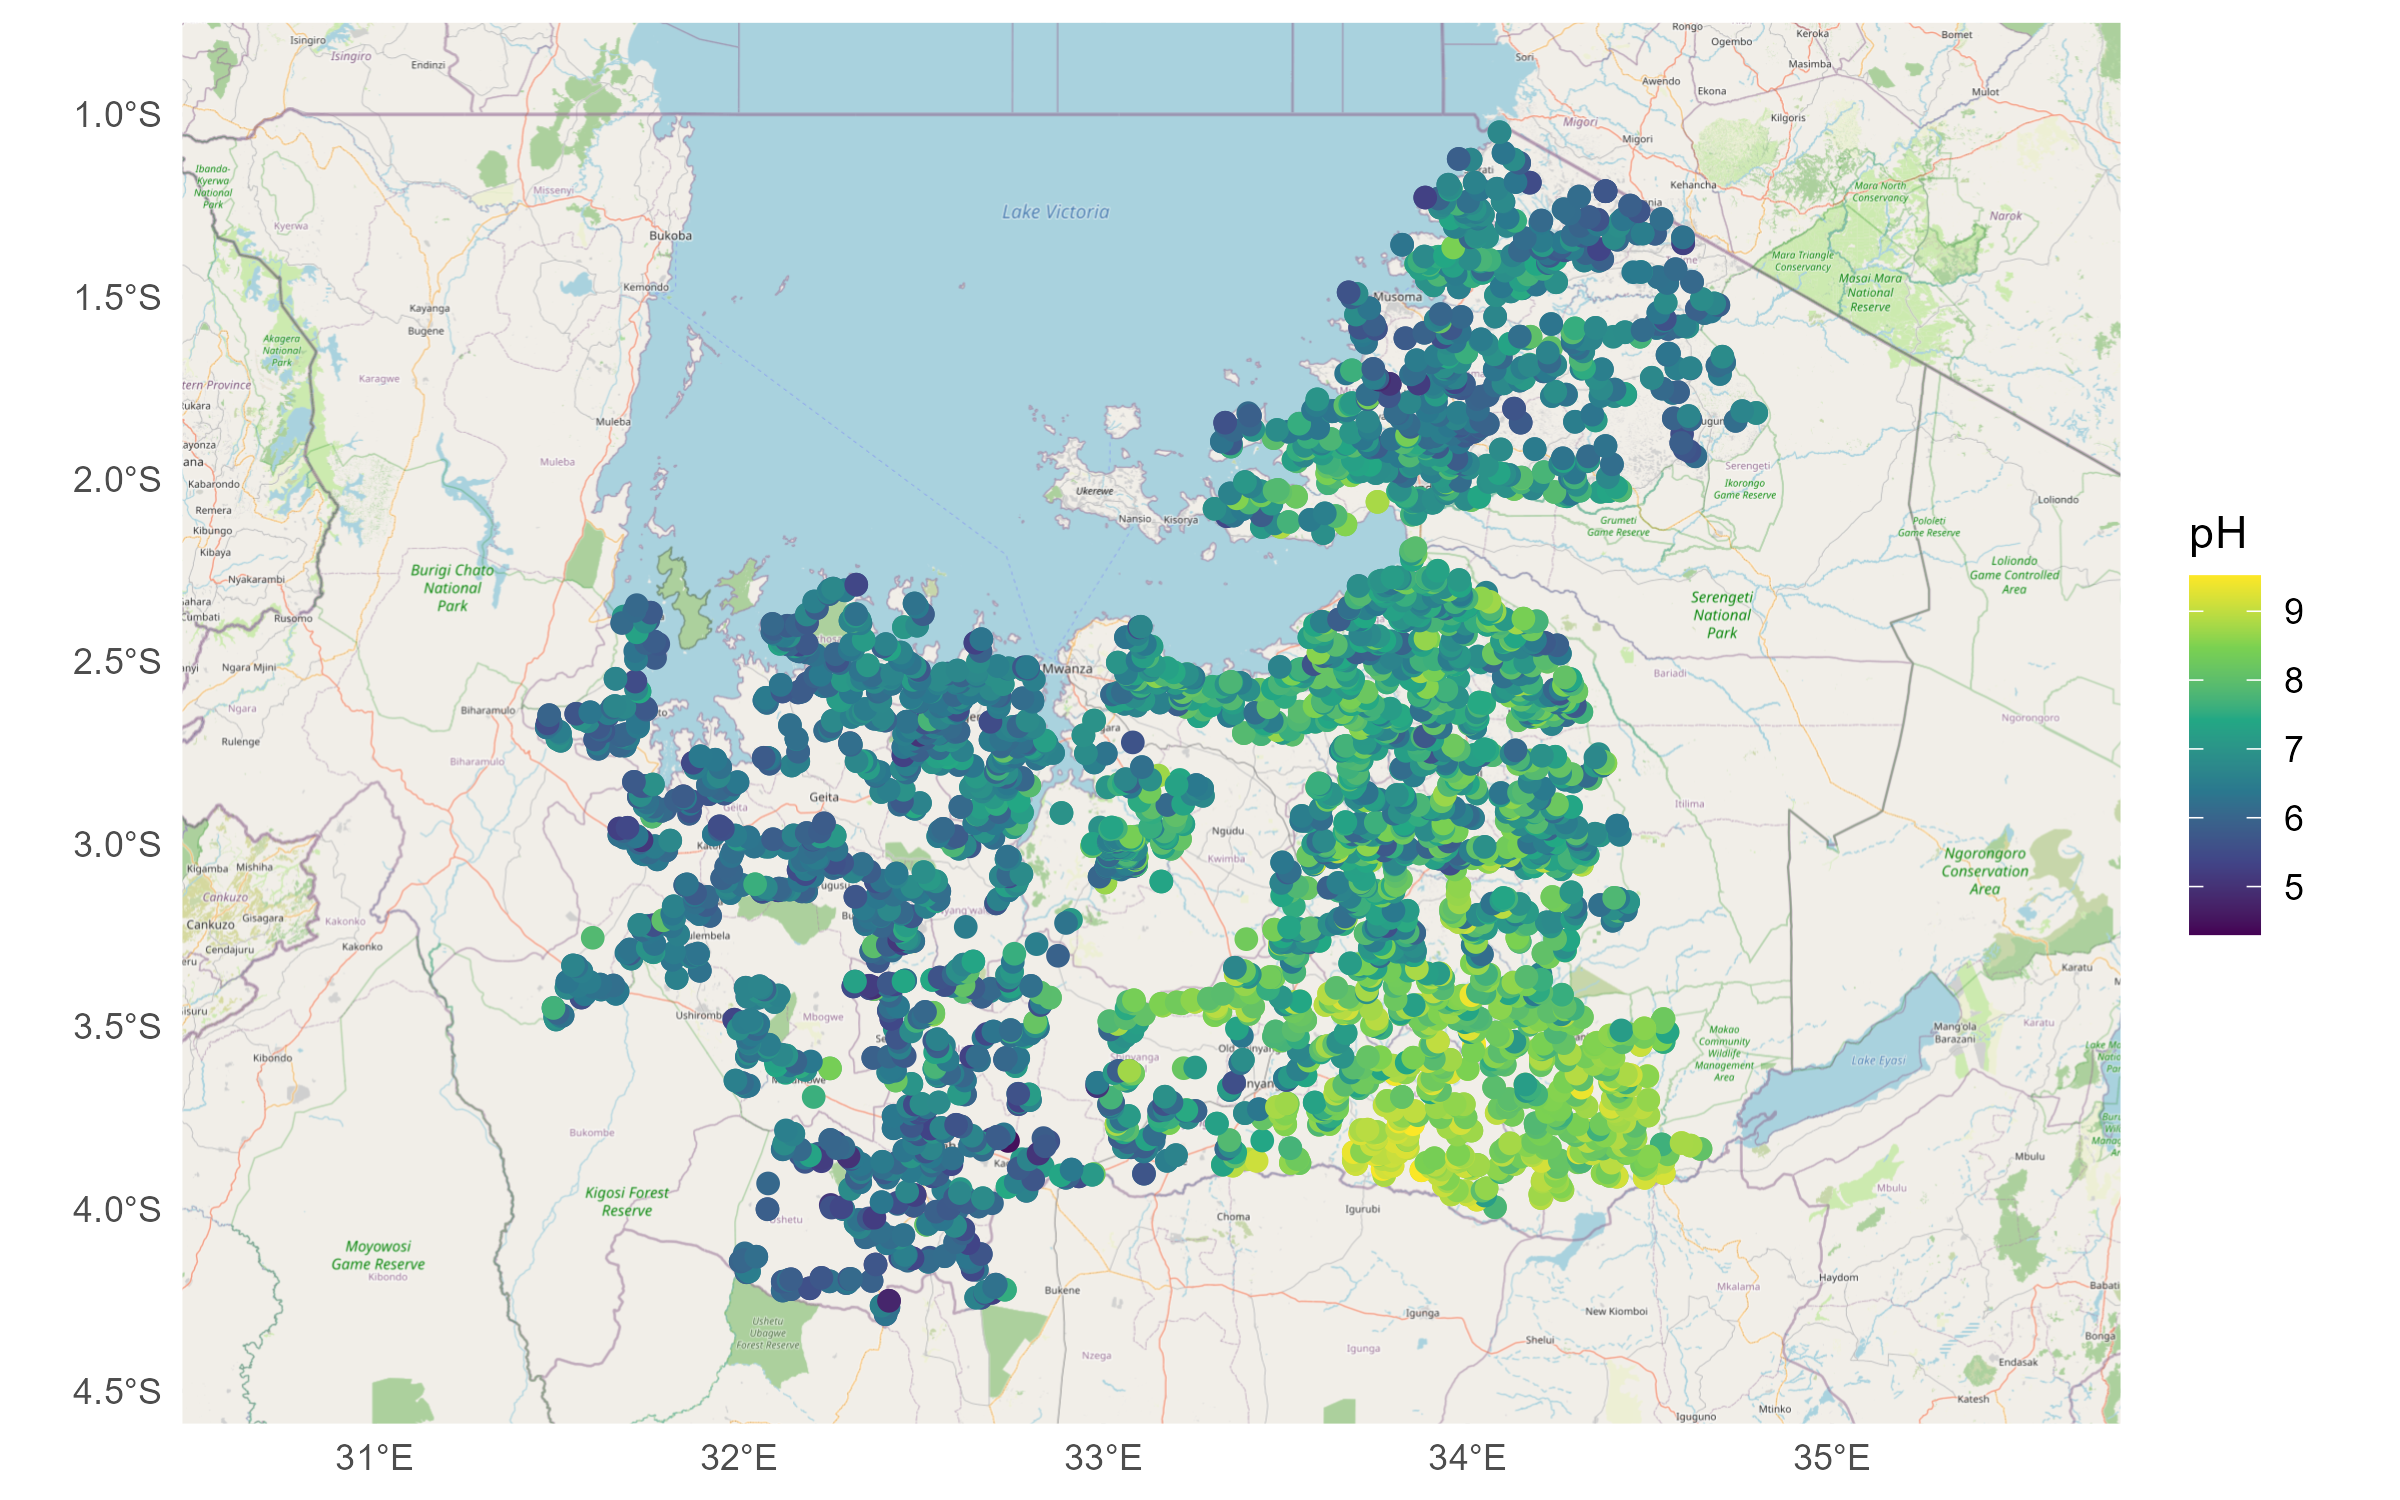
\includegraphics[width=0.5\textwidth]{figuras/mapa_ph.png}
%     \end{center}
% \end{frame}

\begin{frame}{Aplicação em dados reais}
    \begin{itemize}
        \item Encontramos a base de dados "African open soil data" feita pela empresa sem fins-lucrativos iSDA (Innovative Solutions for Decision Agricultured);
        \item Esse empresa cria modelos baseado em AI com o intuito impulsionar a renda de fazendeiros de micro-escala;
        \item Ideia da nossa aplicação e modelar o nível de pH em uma região;
        \item Embora já tenha sido aplicado redes neurais nesses dados, pelo que saibamos, nunca foi aplicado NN-GLS.
    \end{itemize}
\end{frame}
\begin{frame}{Dados}

    \begin{columns}[c]
        \column{0.56\textwidth}

        \begin{itemize}
            \item Nos delimitamos as regiões: Mwanza, Geita, Simiyu, Mara e Shinyanga;
            \item Variável resposta: pH;
            \item Covariáveis: Carbono, Nitrogênio, Alumínio, Cálcio, Cobre, Ferro, Manganês, Magnésio, Potássio, Latitude e Longitude.
        \end{itemize}

        \column{0.44\textwidth}
        \centering
        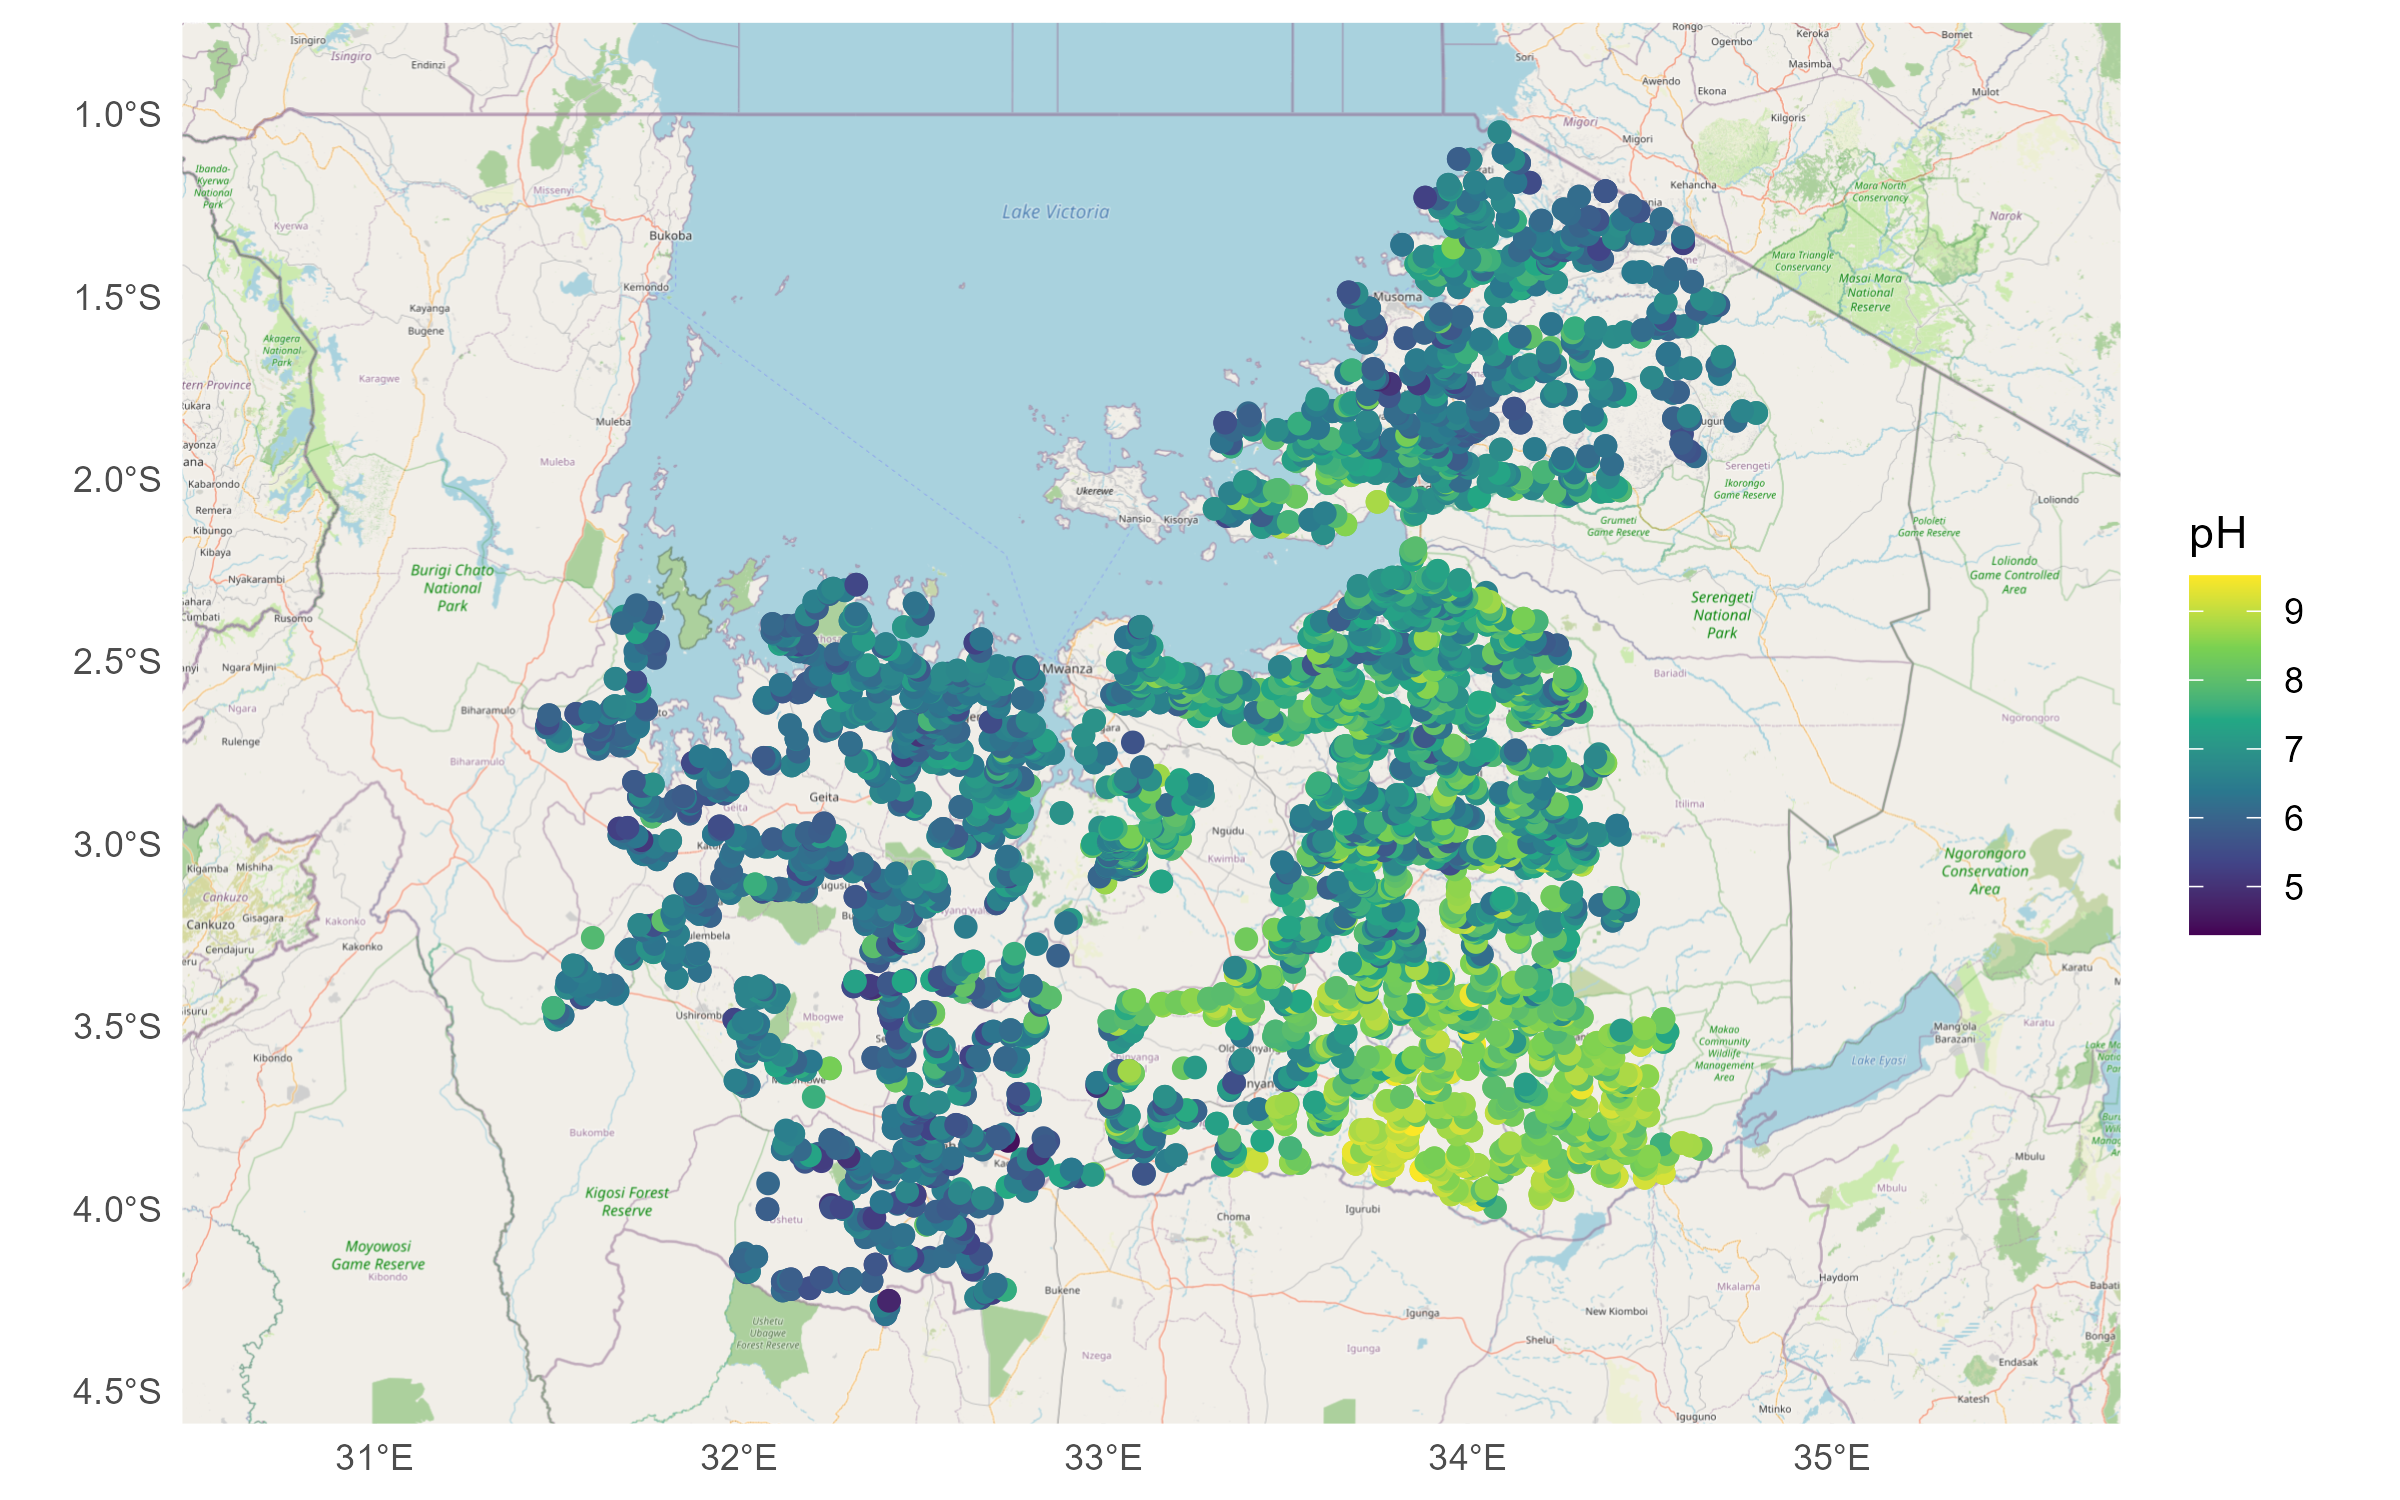
\includegraphics[width=\linewidth]{figuras/mapa_ph.png}
    \end{columns}
\end{frame}


% \begin{frame}{Histogramas}
%     \begin{center}
%         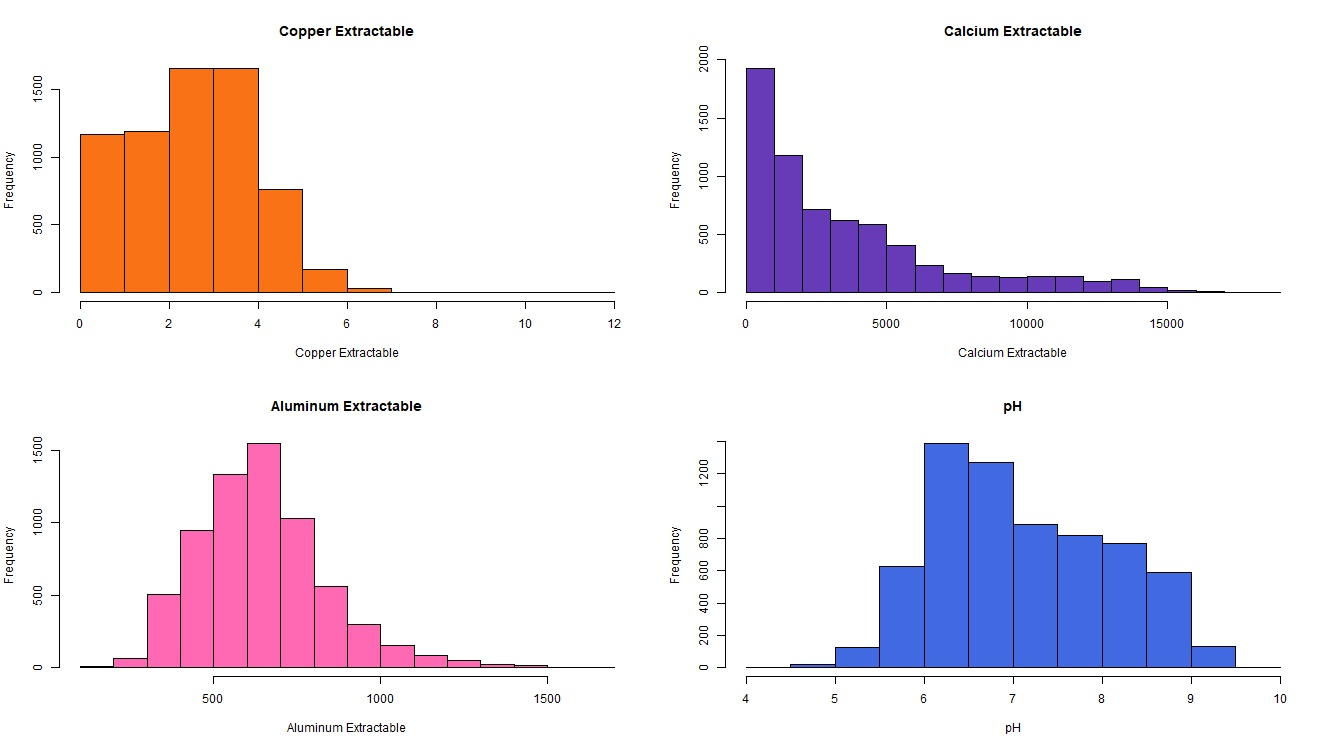
\includegraphics[width=\textwidth]{figuras/hist_lado2.jpg}
%     \end{center}
% \end{frame}

\begin{frame}{Histogramas}
    \begin{center}
        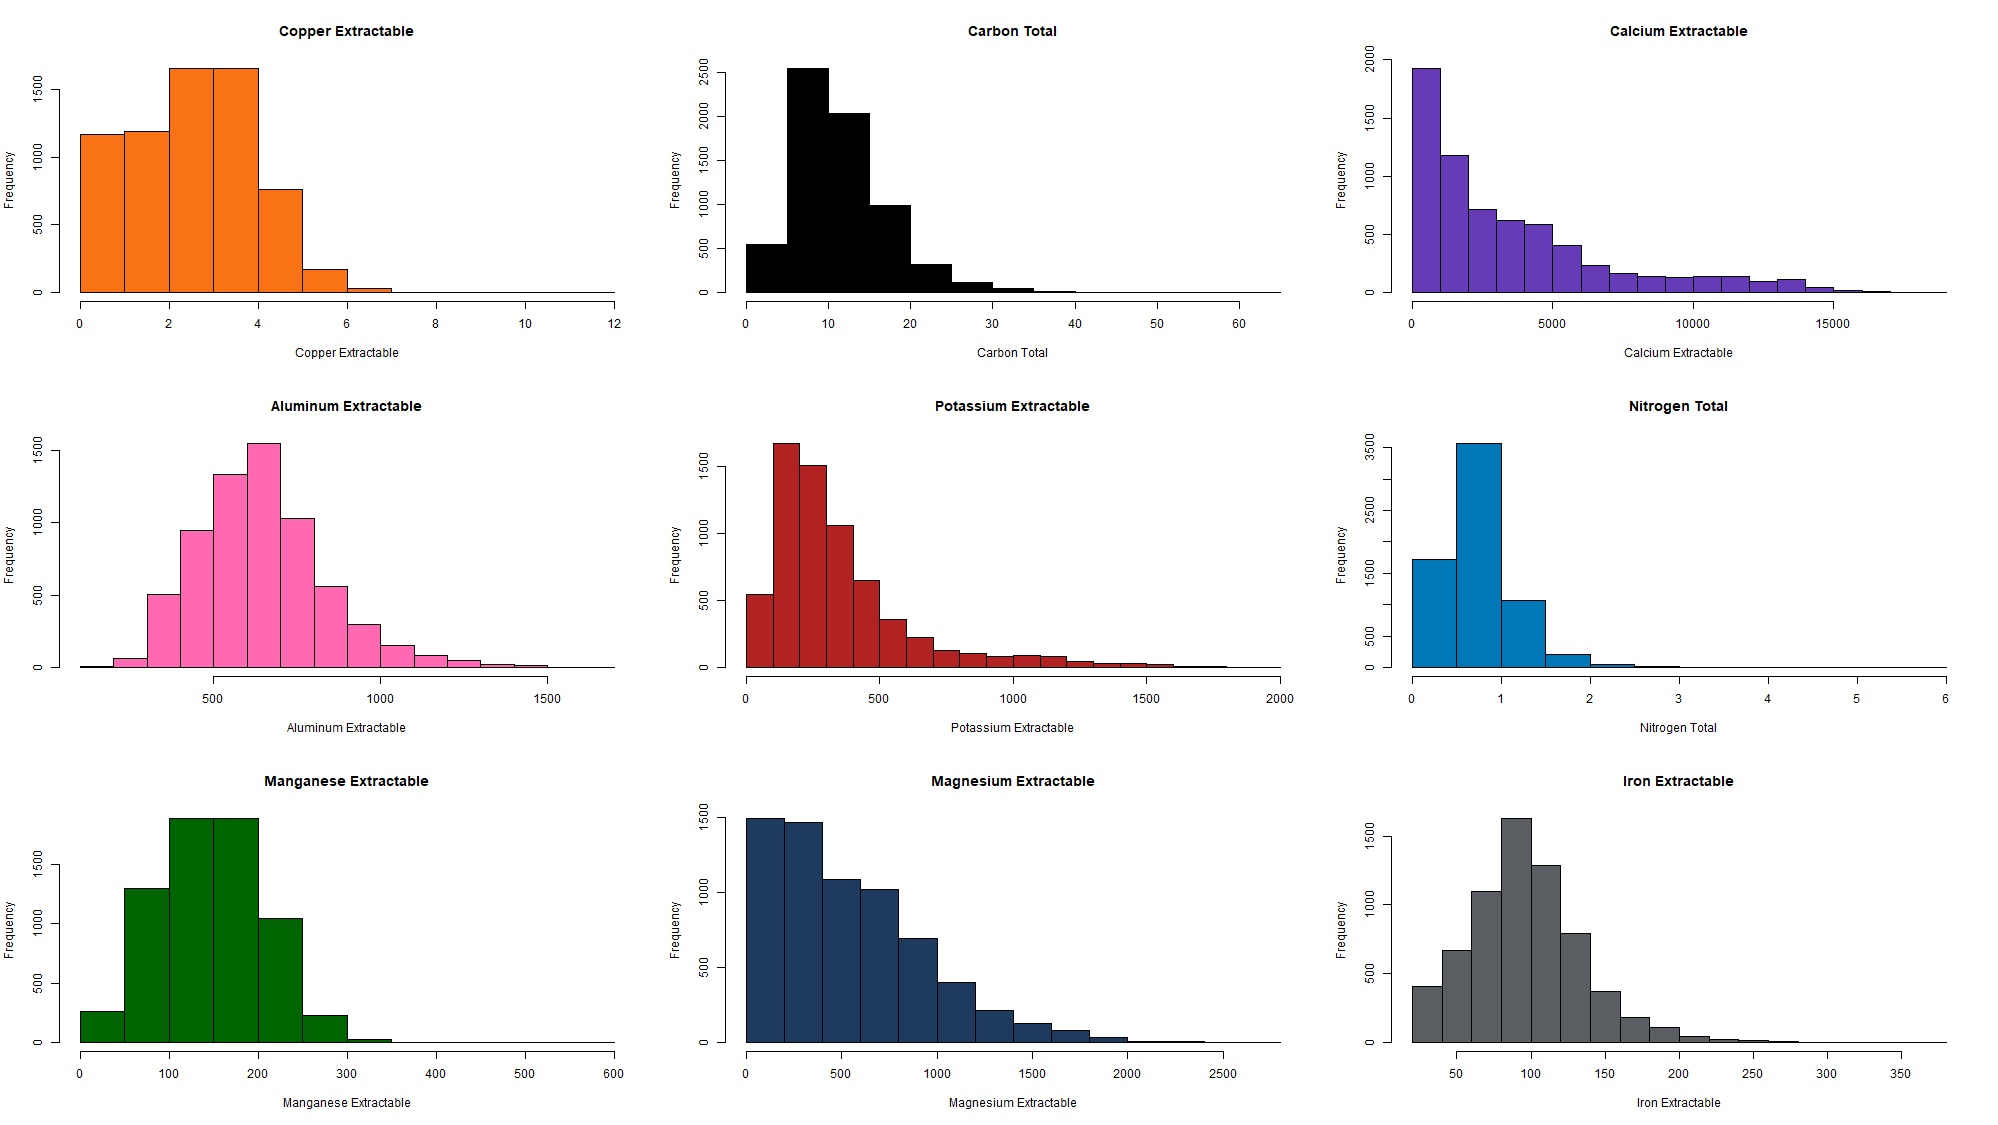
\includegraphics[width=\textwidth]{figuras/hist_lado3.jpg}
    \end{center}
\end{frame}

\begin{frame}{Histogramas}
    \begin{table}[htbp]
        \centering
        \renewcommand{\arraystretch}{1.2}
        \caption{Comparação de Desempenho e Parâmetros dos Métodos de Estimação}
        \label{tab:comparacao_inla_brisc}
        \begin{tabular}{@{}lccccc@{}}
            \toprule
            Método & Tempo & $\sigma^2$ & $\phi$ & $\tau^2$ & EQM \\
            \midrule
            INLA & 1 min 16 s & 0.01849 & 0.111 & 3.82719 & 0.07797 \\
            BRISC & 42 s & 0.05974 & 0.104 & 1.37450 & 0.10522 \\
            Vero. Completa & 22 min 2 s & 0.05485 & 0.13075 & 1.57582 & 0.11426 \\
            \bottomrule
        \end{tabular}
    \end{table}

    \begin{figure}[htbp]
    \centering
    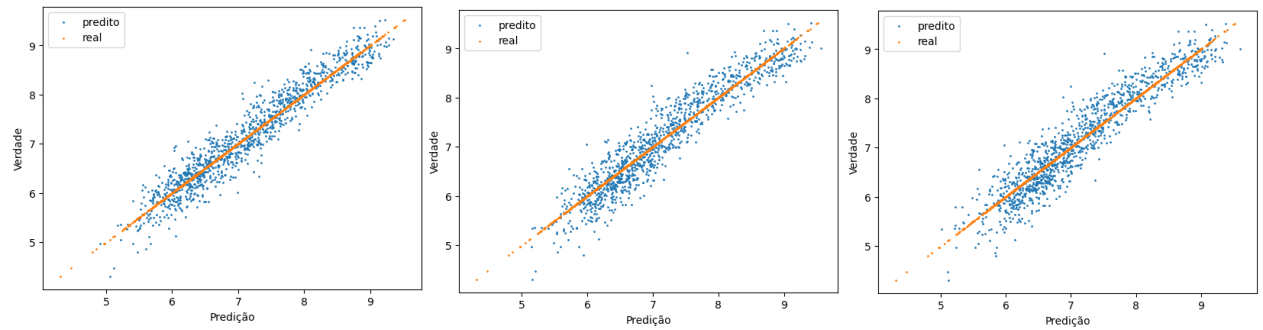
\includegraphics[width=1\textwidth]{figuras/EQM_triples.png}
    \caption{Gráfico de comparação dos valores reais contra preditos, na esquerda INLA, no meio BRISC e na direita vero. completa.}
    \label{fig:EQM_triples}
    \end{figure}

\end{frame}

\begin{frame}
    \begin{figure}[htbp]
        \centering
        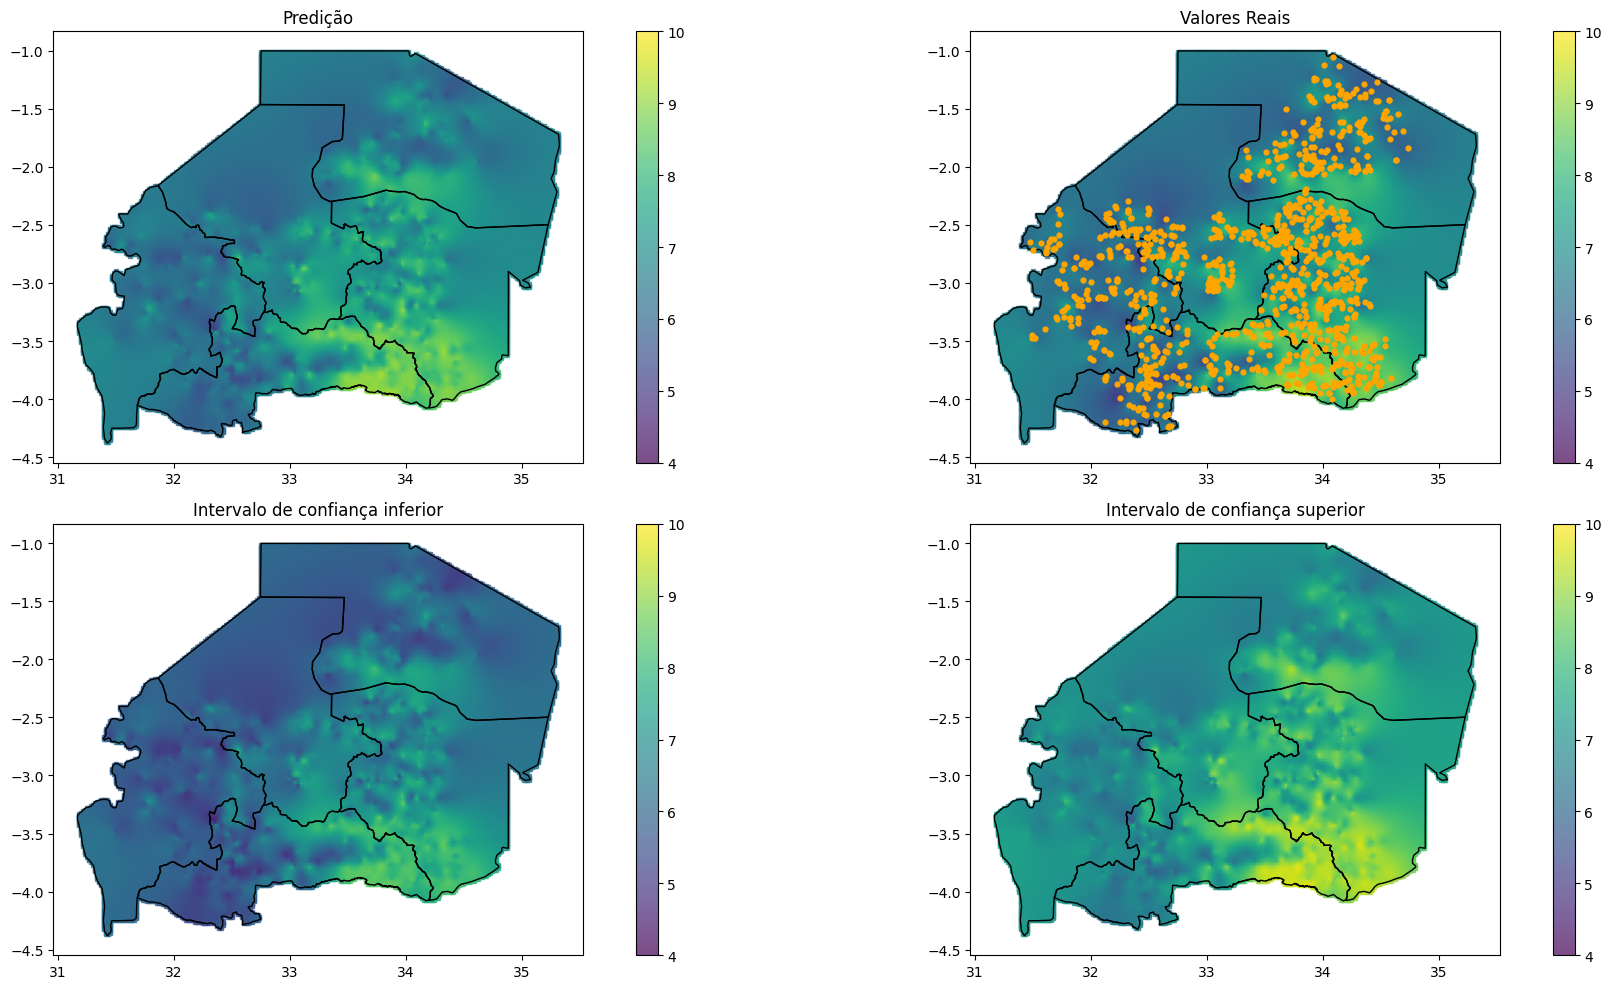
\includegraphics[width=\textwidth,height=\textheight,keepaspectratio]{figuras/Predicao_bayes.png}
        \caption{Krigagem Ordinária com do método Bayesiano}
        \label{fig:pred_bayes}
    \end{figure}
\end{frame}

\begin{frame}
    \begin{figure}[htbp]
        \centering
        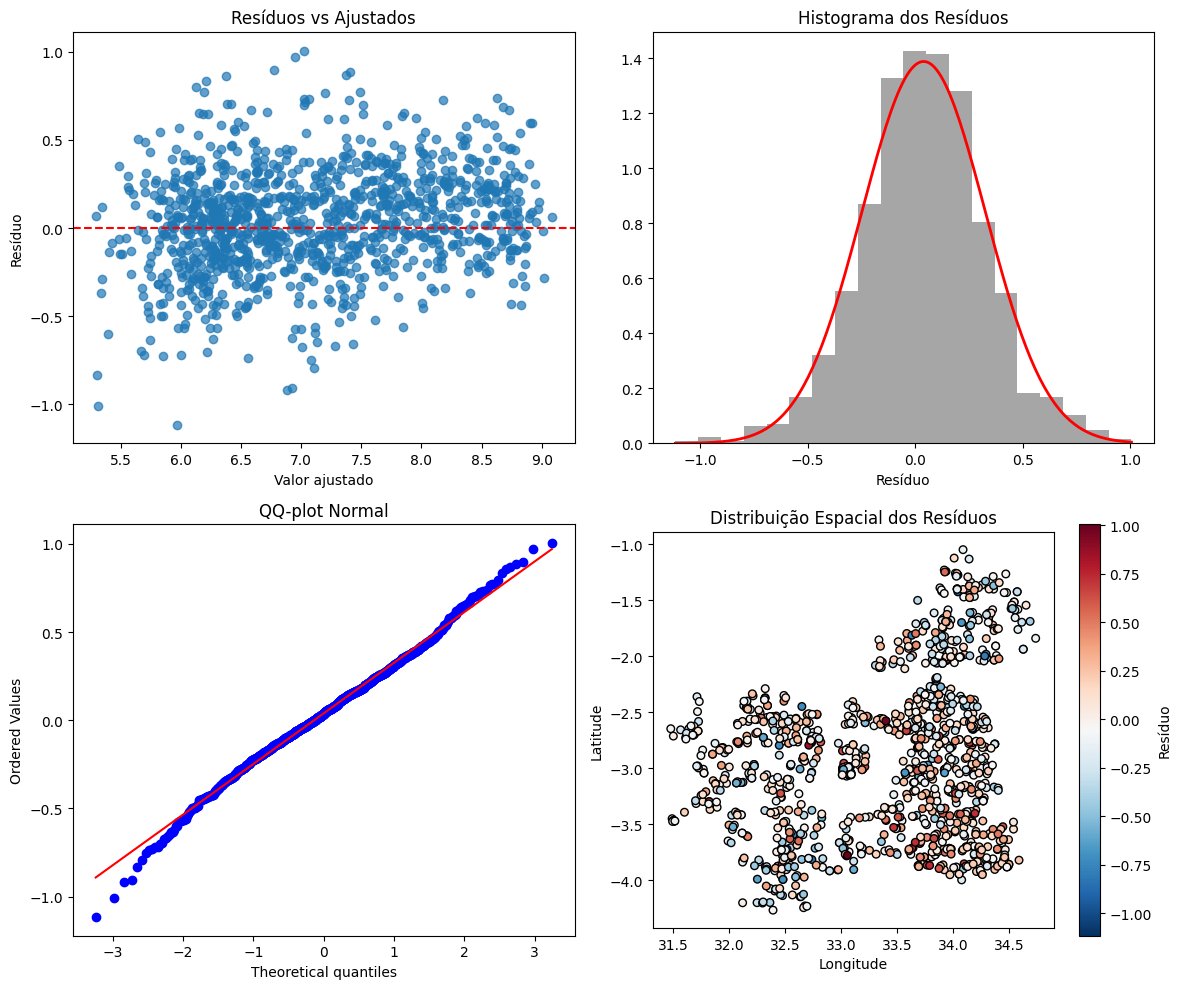
\includegraphics[width=0.75\textwidth,height=\textheight,keepaspectratio]{figuras/residuos_INLA.png}
        \caption{Diagnóstico dos resíduos do modelo NN-GLS com INLA}
        \label{fig:residuos_INLA}
    \end{figure}
\end{frame}

% \begin{frame}{Histogramas}
%     \begin{center}
%         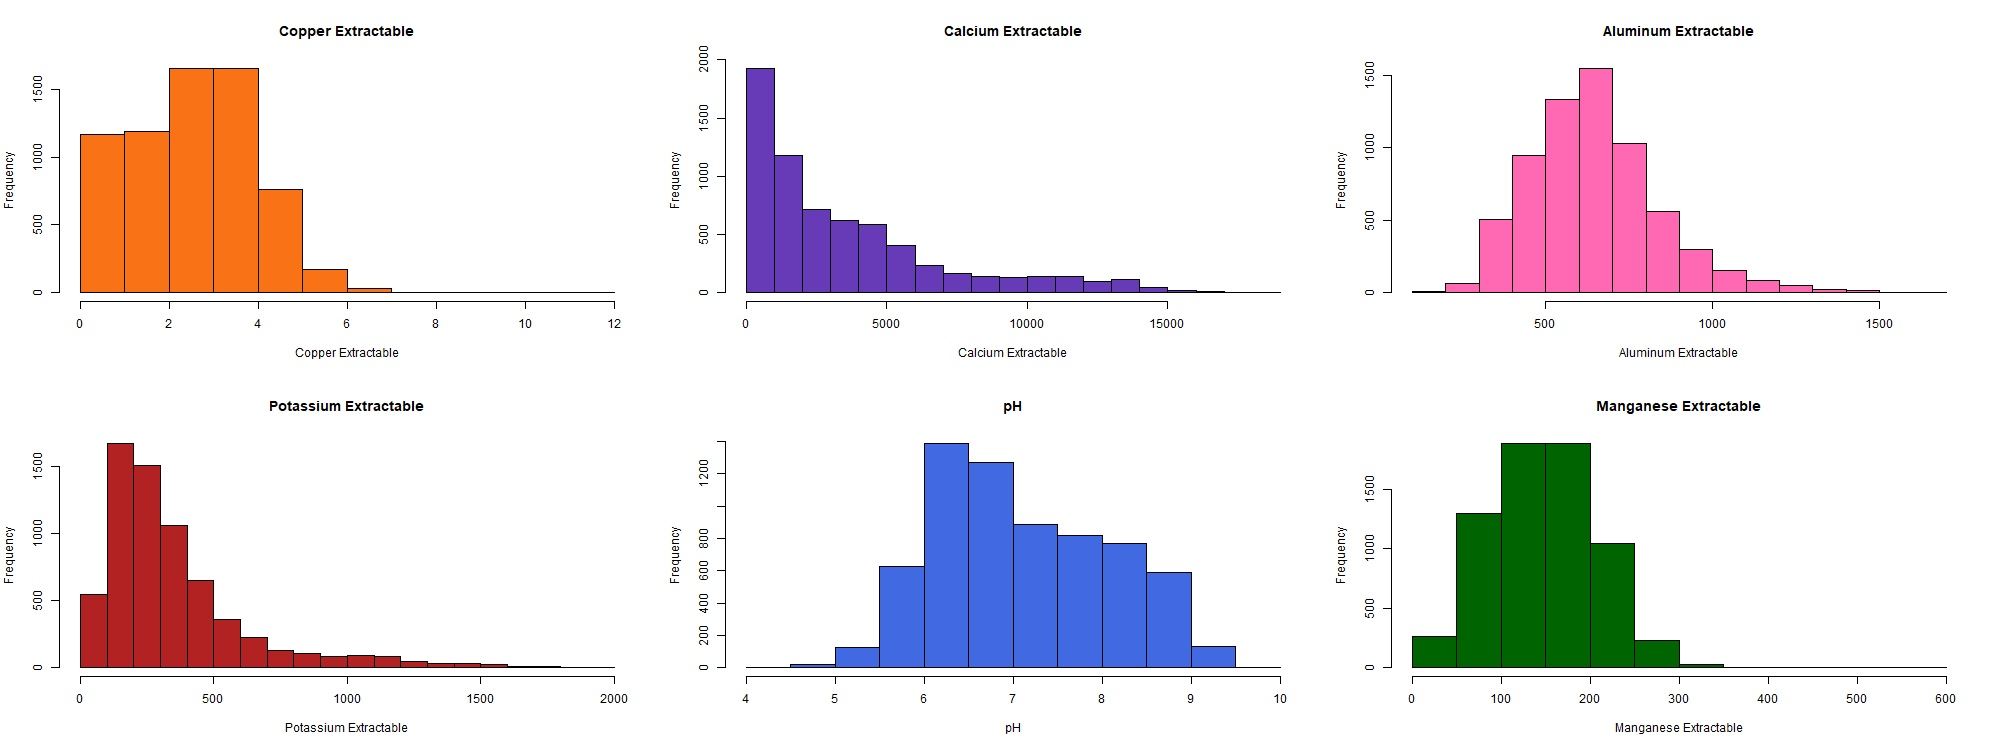
\includegraphics[width=\textwidth]{figuras/hist_lado4.jpg}
%     \end{center}
% \end{frame}





    % =============================================================
    % SEÇÃO 6: CONCLUSÃO
    % =============================================================
    \section{Conclusão}

    \begin{frame}{Conclusões e Trabalhos Futuros}
            \textbf{Conclusões:}
            \begin{itemize}
                \item Eficiência de cada método está diretamente relacionada à intensidade da dependência espacial presente nos dados;
                \item INLA foi mais vantajoso em cenários com dependência espacial baixa;
                \item Escolha do método deve levar em conta a natureza dos parâmetros.
            \end{itemize}
        \textbf{Trabalhos Futuros:}
        \begin{itemize}
            \item Simulações com anisotropia e dupla tendência;
            \item Testar outras prioris;
            \item Modificar de outra forma o conjunto de condicionamento.
        \end{itemize} 
    \end{frame}

    % -------------------------------------------------------------
    % SLIDE: AGRADECIMENTOS
    % -------------------------------------------------------------
    \begin{frame}{Agradecimentos}
        \begin{center}
            \vspace{1cm}
            {\Large \textbf{Obrigado pela atenção!}}
            
            \vspace{0.8cm}
            \textbf{Yuri Dessimon} \\
            \texttt{yuri.dessimon@ufrgs.br}
            
            \vspace{0.5cm}
            \small Instituto de Matemática e Estatística (IME) \\
            Universidade Federal do Rio Grande do Sul (UFRGS)
        \end{center}
    \end{frame}

    \end{document}

